% \chapter{Materials}\label{chp:materials}
\chapter{材料}
\label{chp:materials}
% \section{Introduction}
\section{简介}
% This chapter provides essential information on materials used for constructing durable bridge structures. It focuses on durability and service life issues related mainly to concrete and steel, materials widely used in bridge construction, and provides limited information on other material types used in bridge construction.
本章提供有关用于建造耐用桥梁结构的材料的基本信息。它侧重于与桥梁建设中广泛使用的混凝土和钢材相关的耐久性和\gls*{servicelife}问题,并提供有关桥梁建设中使用的其他材料类型的有限信息。

% Information for enhancing the service life of materials used in bridge systems, subsystems, and components is summarized. \cref{fig:mat-enhance-selection-process} identifies the materials-enhancement selection process used, and this chapter follows the structure of that process which begins with developing an understanding of the types of materials. These viable materials are further evaluated for the factors that adversely affect their service life. Individual strategies are then developed to mitigate these adverse effects. The overall strategy selection is then developed, blending these individual strategies that are sometimes in conflict with each other. The components of an overall strategy should:
在此总结了用于提高桥梁\gls*{system}、\gls*{subsystem}和\gls*{component}所用材料\gls*{servicelife}的信息。\cref{fig:mat-enhance-selection-process} 显示了所使用的材料优选过程,该过程从理解材料类型开始,本章内容则遵循该过程的结构。 这些可行的材料将进一步评估对其\gls*{servicelife}产生不利影响的因素,然后制定单独的策略来减轻这些不利影响,然后制定总体策略的选择,融合这些有时相互冲突的个别策略。 总体战略的组成部分应该:

% \begin{itemize}
  % \item Identify appropriate design methodologies;
  % \item Select durable material types considering life cycle costs;
  % \item Consider additional protective measures, such as cathodic protection and electrochemical chloride extraction;
  % \item Specify best practices for construction; and
  % \item Develop an effective maintenance plan.
% \end{itemize}
\begin{itemize}
  \item 确定适当的设计方法;
  \item 考虑生命周期成本选择耐用材料类型;
  \item 考虑额外的保护措施,例如阴极保护和电化学方法提取氯化物;
  \item 指定施工的最佳工法;
  \item 制定有效的维护计划。
\end{itemize}

\begin{figure}
  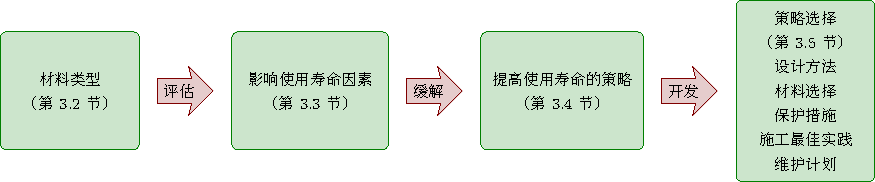
\includegraphics{mat-enhance-selection-process.pdf}
  \caption{材料优选过程}\label{fig:mat-enhance-selection-process}
\end{figure}

% \cref{sec:material-types} provides a general description of material types used for bridge systems, subsystems, and components, primarily concrete, reinforcement, and structural steel. \cref{sec:concrete-steel-distresses-solutions}addresses factors known to adversely affect service life of these materials and Section 3.4 presents a fault tree approach for considering these factors. Section 3.5 provides available solutions, methods, technologies, and other information helpful in developing individual strategies to mitigate factors adversely affecting service life. Section 3.6 identifies a process to select the overall material selection and protection strategy for providing materials with enhanced service life; however, much of this selection process is highly dependent on the application and is addressed in subsequent chapters.
\cref{sec:material-types}提供了用于桥梁\gls*{system}、\gls*{subsystem}和\gls*{component}的材料类型的一般描述,主要是混凝土、钢筋和结构钢。 \cref{sec:concrete-steel-distresses-solutions}阐述了已知对这些材料的\gls*{servicelife}产生不利影响的因素,\cref{sec:factor-influence-fault-tree}介绍了考虑这些因素的{故障树}方法。\cref{sec:individual-strategies}提供了可用的解决方案、方法、技术和其他有助于制定单独策略以减轻对使用寿命产生不利影响的因素的信息。 \cref{sec:overall-strategies}确定了选择整体材料选择和保护策略的过程,以提供具有更长使用寿命的材料; 然而,这个选择过程的大部分高度依赖于应用,并在后续章节中讨论。

% \section{Description of Material Types}
\section{材料类型的说明}
\label{sec:material-types}

% This section provides a general description of the materials used for bridge systems, subsystems, and components, primarily concrete, reinforcement and structural steel.
本节提供了用于桥梁\gls*{system}、\gls*{subsystem}和\gls*{component}的材料的一般描述,主要是混凝土、钢筋和结构钢。

% Different concretes for bridge elements require different degrees of durability depending on the exposure environment and the properties desired. There are many examples of longevity of concrete from ancient times, for example the Pantheon in Rome, which was built around 126 A.D. and remains intact. The Confederation Bridge, which joins the eastern Canadian provinces of Prince Edward Island and New Brunswick, was constructed in 1997 and is a good example of a modern concrete bridge designed to resist the harsh marine environment for at least 100 years (\cref{fig:confederation-bridge}).
用于桥梁\gls*{element}的不同混凝土需要不同程度的耐久性,具体取决于所处的暴露环境和所需的特性。古代有许多混凝土经久不衰的例子,例如罗马的万神殿,它建于公元 126 年左右,至今仍完好无损。联邦大桥连接加拿大东部省份爱德华王子岛省和新不伦瑞克省,建于 1997 年,其设计目标是能在至少 100 年内抵御恶劣的海洋环境,是现代混凝土桥梁的典范(\cref{fig:confederation-bridge})。

\begin{figure}
  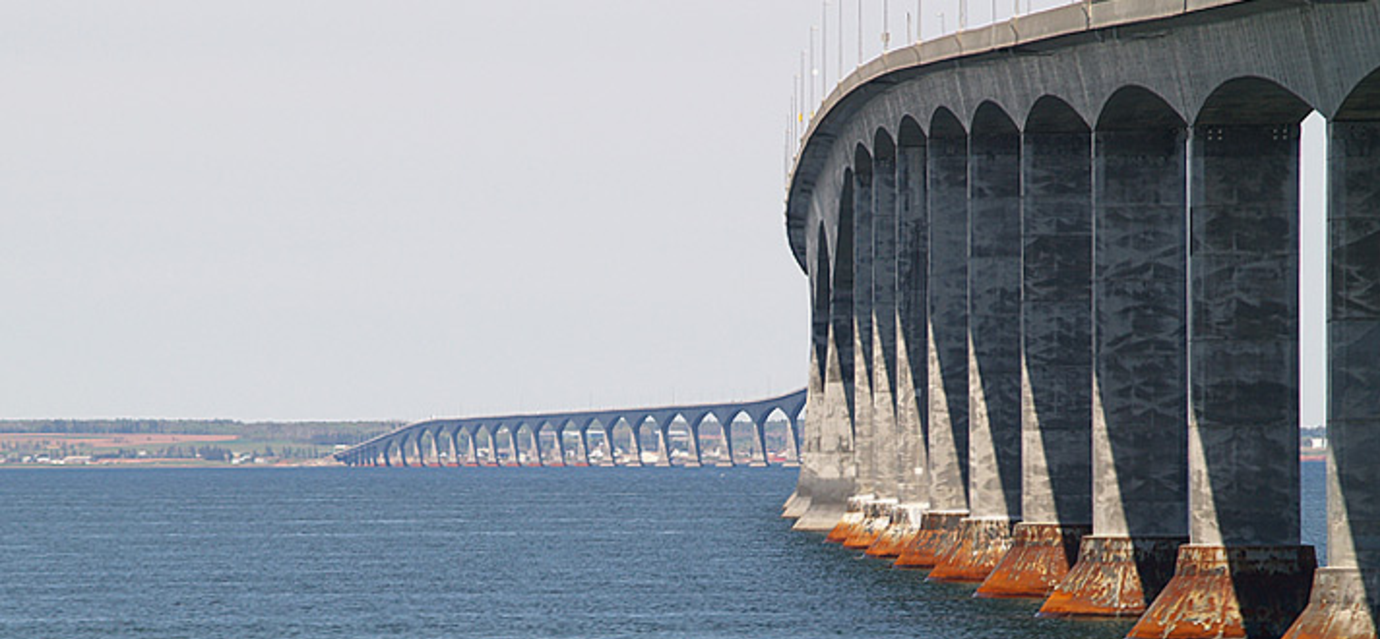
\includegraphics[width=\linewidth]{confederation-bridge.png}
  \caption{Confederation Bridge}\label{fig:confederation-bridge}
\end{figure}

% Concrete has high compressive, but low tensile strength, which makes it prone to cracking. Early concrete structures were designed to be subjected only to compression, thereby avoiding tensile failures. Arch shapes were used to span distances. In modern structures, reinforcement is common for providing tensile capacity, crack control, and ductility. The service life of reinforced concrete structures depends on the durability of concrete and the durability of the reinforcement.
混凝土的抗压强度高,但抗拉强度低,容易开裂。早期的混凝土结构设计为仅受压,从而避免拉伸破坏。需要跨越较大的距离时则采用拱结构。在现代结构中,钢筋通常用于提供抗拉能力、裂缝控制和构件延性。钢筋混凝土结构的\gls*{servicelife}取决于混凝土的耐久性和钢筋的耐久性。

% The major distress in reinforced concrete is due to the corrosion of the reinforcement. Reinforcement must be protected from aggressive environments either through measures such as the use of the low permeability concrete, adequate cover, and corrosion inhibitors, or the use of noncorrosive reinforcement. Preventive measures could also be employed to prolong the service life of concrete structures, such as incorporating cathodic protection systems.
钢筋混凝土的主要缺陷在于钢筋的腐蚀。必须通过使用低渗透性混凝土、足够的保护层、添加腐蚀抑制剂或使用抗腐蚀钢筋等措施,保护钢筋免受侵蚀性环境的影响。还可以采用预防措施来延长混凝土结构的\gls*{servicelife},例如采用阴极保护系统。

% Structural steel is another common material used for bridge systems, subsystems, and components. It provides high compressive and tensile strengths with considerable ductility, which makes it particularly suitable for long-span bridges. The most common steel bridge systems used today are composite multi-girder deck systems which use either rolled beams, plate girders, or tub girders. These systems can be single- or multi-span, and either straight or curved. Simple-span systems were often used in the past, but most multi-span systems today are continuous. Rolled beam bridges using W-shapes are used in shorter spans up to about 100 ft for simple-spans and up to about 120 ft for continuous spans. Welded deck plate girders are most often used for spans over 120 ft.
结构钢是另一种用于桥梁\gls*{system}、\gls*{subsystem}和\gls*{component}的常用材料。它提供较高的抗压和抗拉强度以及相当大的延展性,这使得它特别适用于大跨度桥梁。当今使用的最常见的钢桥系统是组合多梁桥面系统,它使用轧制梁、板梁或槽形梁。 这些系统可以是单跨或多跨,可以是直的也可以是弯的。过去经常使用简支体系,但如今大多数多跨体系都是连续的。W 形的轧制梁桥用于较短的跨度,简支梁跨径可达约 \qty{30}{m},连续梁跨径可达约 \qty{35}{m}。 焊接钢板梁最常用于 \qty{35}{m} 以上的跨径。

% \subsection{Concrete}
\subsection{混凝土}
% Concrete consists of cementitious material, aggregate, water, and admixtures. Concrete may also include fibers. The following sections provide general descriptions of each concrete ingredient.
混凝土由胶凝材料、骨料、水和外加剂组成。混凝土还可以包括纤维。以下部分提供了每种具体成分的一般描述。

% \subsubsection{Cementitious Material}
\subsubsection{胶凝材料}
% Cementitious materials include portland cements, blended cements, other hydraulic cements, specialty cements for repairs, and supplementary cementitious materials (SCM). These cementitious materials have different chemical and physical properties that affect the durability of concrete.
胶凝材料包括硅酸盐水泥、混合水泥、其他水硬性水泥、用于修复的特种水泥和\acrfull*{scm}。 这些胶凝材料具有影响混凝土耐久性的不同物理化学特性。

% \paragraph{Portland Cement}
\paragraph{波特兰水泥}
% Portland cement is produced from a combination of calcium, silica, aluminum, and iron (Kosmatka and Wilson 2011). The raw materials reach temperatures of 2600ºF to 3000ºF, forming clinker. Clinker and gypsum are ground to a fine powder such that nearly all of it passes a No. 200 mesh (75micron sieve). Cement has four main compounds: tricalcium silicate (3CaO.SiO2=C3S), dicalcium silicate (2CaO.SiO2=C2S), tricalcium aluminate (3CaO.Al2O3=C3A), and tetracalcium aluminaferrite (4CaO.Al2O3. Fe2O3=C4AF). These form the different types of portland cements conforming to the requirements of \acrshort*{astm} C150. Ten types of portland cement are summarized in {tab:cement-types}.
波特兰水泥由钙、二氧化硅、铝和铁的混合物制成 \cite{kosmatka2011d}。 原材料加热到 \qtyrange{1400}{1600}{\celsius} 的温度形成熟料,熟料和石膏被研磨成细粉,几乎所有粉末都可以通过 200 目(\qty{75}{\micro m} 筛)。水泥有四种主要化合物:
% 硅酸三钙(\ce{3CaO.SiO2=C3S})、
% 硅酸二钙(\ce{2CaO.SiO2=C2S})、
% 铝酸三钙(\ce{3CaO.Al2O3=C3A})和铁酸铝四钙(\ce{4CaO.Al2O3.Fe2O3=C4AF})。
\begin{itemize}
  \item 硅酸三钙(\ce{3CaO.SiO2=C3S});
  \item 硅酸二钙(\ce{2CaO.SiO2=C2S});
  \item 铝酸三钙(\ce{3CaO.Al2O3=C3A});
  \item 铁酸铝四钙(\ce{4CaO.Al2O3.Fe2O3=C4AF})。
\end{itemize}
这些形成符合 \acrshort*{astm} C150 要求的不同类型的波特兰水泥。\cref{tab:cement-types} 中总结了十种硅酸盐水泥。

\begin{table}
  \caption{水泥种类与用途}\label{tab:cement-types}
  \begin{tblr}{
  colspec={X[l] X[l,3]},
  row{1}={bg=genfg,fg=white,font=\bfseries}
}
水泥类型     & 使用   \\
类型 I       & 一般用途  \\
类型 IA      & 类型 I + 引气  \\
类型 II      & 一般用途,中等抗硫酸盐性  \\
类型 IIA     & 类型 II + 引气  \\
类型 II(MH)  & 一般用途,中等水化热,中等抗硫酸盐性  \\
类型 II(MH)A & 类型 II(MH) + 引气  \\
类型 III     & 早期强度高  \\
类型 IIIA    & 类型 III + 引气  \\
类型 IV      & 低水化热  \\
类型 V       & 高抗硫酸盐性  \\
\end{tblr}
\end{table}

% Some cements are designated with a combined classification, such as Type I/II indicating that cement meets all of the requirements of the specified types.
一些水泥被指定为组合分类,例如类型 I/II 表示水泥满足特定类型的所有要求。

% \paragraph{Blended Cement}
\paragraph{混合水泥}
% Blended cements are produced by intergrinding or blending two or more types of fine material such as portland cement, ground granulated blast furnace slag, fly ash, silica fume, calcined clay, other pozzolans, hydrated lime, and pre-blended combinations of these materials \cite{kosmatka2011d}. \acrshort*{astm} C595 includes three classes of blended cement:
混合水泥是通过共同研磨或混合两种或多种精细材料生产的,例如波特兰水泥、磨碎的粒状高炉矿渣、粉煤灰、硅灰、煅烧粘土、其他火山灰、熟石灰,以及这些材料的预混合组合  \cite{kosmatka2011d}。\acrshort*{astm} C595 包括三类混合水泥:

% \begin{itemize}
%   \item Type IS (X)—Portland blast furnace slag cement
%   \item Type IP (X)—Portland-pozzolan cement
%   \item Type IT(AX)(BY)—Ternary blended cement
% \end{itemize}
\begin{itemize}
  \item 类型 IS(X)—波特兰高炉矿渣水泥
  \item 类型 IP(X)—波特兰火山灰水泥
  \item 类型 IT(AX)(BY)—三元混合水泥
\end{itemize}

% The letters X and Y stand for the percentage of SCM included in the blended cement, and A and B are the Types of SCMs, either S for slag or P for pozzolan. Type IS(X) can include up to 95\% slag cement. Type IP(X) can include up to 40\% pozzolans. Special properties are designated as follows, and added after the percentages. For example: IP(25)(HS) indicates 25\% pozzolans and high sulfate resistance.
字母 X 和 Y 代表混合水泥中\acrlong*{scm}的百分比,A 和 B 是\acrlong*{scm}的类型,取 S 代表矿渣或取 P 代表火山灰。IS(X) 型可包含高达 95\% 的矿渣水泥。 IP(X) 型可包含高达 40\% 的火山灰。 特殊属性添加在百分比之后。 例如:IP(25)(HS) 表示 25\% 火山灰和高抗硫酸盐性。

% \begin{itemize}
%   \item Air entrainment—(A)
%   \item Moderate sulfate resistance—(MS)
%   \item High sulfate resistance—(HS)
%   \item Moderate heat of hydration—(MH)
%   \item Low heat of hydration—(LH)
% \end{itemize}
\begin{itemize}
  \item 引气—(A)
  \item 中等抗硫酸盐性—(MS)
  \item 高抗硫酸盐性—(HS)
  \item 中等水化热—(MH)
  \item 低水化热—(LH)
\end{itemize}

% As an example for ternary cements, Type IT(S25)(P15) contains 25\% slag and 15\% pozzolans. Type IT can meet MS, HS, and LH options.
以三元水泥为例,IT(S25)(P15) 型包含 25\% 的矿渣和 15\% 的火山灰。 IT 型可以满足 MS、HS 和 LH 选项。

% \paragraph{Other Hydraulic Cement}
\paragraph{其他水硬性水泥}
% All portland and blended cements are hydraulic cements. \acrshort*{astm} C1157, is a performance specification that includes portland cement, modified portland cement (specialty cement providing characteristics of more than one type of portland cement), and blended cements. \acrshort*{astm} C1157 recognizes six types of hydraulic cements:
所有波特兰水泥和混合水泥都是水硬性水泥。\acrshort*{astm} C1157 规定了材料的性能,包括硅酸盐水泥、改性硅酸盐水泥(提供不止一种硅酸盐水泥特性的特种水泥)和混合水泥。 \acrshort*{astm} C1157 认可六种水硬性水泥:
% \begin{itemize}
%   \item Type GU --- general use;
%   \item Type HE --- high early strength;
%   \item Type MS --- moderate sulfate resistance;
%   \item Type HS --- high sulfate resistance;
%   \item Type MH --- moderate heat of hydration; and
%   \item Type LH --- low heat of hydration.
% \end{itemize}
\begin{itemize}
  \item 类型 GU — 一般用途;
  \item 类型 HE — 早期强度高;
  \item 类型 MS — 中等抗硫酸盐性;
  \item 类型 HS — 高抗硫酸盐性;
  \item 类型 MH — 中等水化热;
  \item 类型 LH — 低水化热。
\end{itemize}

% \paragraph{Expansive Cements}
\paragraph{膨胀水泥}
% Expansive cements are modified hydraulic cements that expand slightly during the early hardening period after setting. They are used to compensate for volume decrease due to drying shrinkage, to induce tensile stress in reinforcement, and to stabilize long-term dimensions of post-tensioned concrete. \acrshort*{astm} C845 designates E-1 with three varieties—K, M, and S—and only K is available in the United States. Type E-1 (K) contains portland cement, anhydrous tetracalcium trialuminosulfate, calcium sulfate, and uncombined calcium oxide (lime).
膨胀水泥是改性水硬性水泥,在凝固后的早期硬化期间略有膨胀。它们用于补偿由于干燥收缩引起的体积减少,在钢筋中引起拉应力,以及稳定后张预应力混凝土的长期尺寸。 \acrshort*{astm} C845 将 E--1 指定为三个品种——K、M 和 S——在美国只有 K 可用。 E--1 (K) 型包含硅酸盐水泥、无水三铝硫酸四钙、硫酸钙和未化合的氧化钙(石灰)。

% It has been demonstrated that using lightweight aggregate in concrete with expansive cements is very beneficial for achieving the expansion from expansive cements (Russell 1978). This effect is attributed to the continued presence of internal moisture that has been absorbed by the lightweight aggregate prior to batching. This internal moisture allows a prolonged reaction time for the expansive cement, so it achieves greater expansion. Therefore, it is suggested that lightweight aggregate be used in conjunction with expansive cements.
已经证明,在含有膨胀水泥的混凝土中使用轻骨料对于实现膨胀水泥的膨胀非常有利 \cite{russell1978p}。 这种影响归因于在配料之前已被轻骨料吸收的内部水分的持续存在。 这种内部水分可以延长膨胀水泥的反应时间,从而实现更大的膨胀。因此,建议轻骨料与膨胀水泥配合使用。

% \paragraph{Specialty Cements for Repairs}
\paragraph{修复用特种水泥}
% Specialty cements for repairs are needed to achieve high early strengths, and cements other than the portland cements may be used. They may be rapid-setting hydraulic cement, gypsum-based cement, magnesium phosphate cement, or high-alumina cement for use in partial depth concrete repairs (Caltran 2008; ACPA 1998).
需要用于修复的特种水泥来获得高早期强度,并且可以使用硅酸盐水泥以外的水泥。 它们可能是用于局部深度混凝土修复的速凝水凝水泥、石膏基水泥、磷酸镁水泥或高铝水泥 (Caltran 2008; ACPA 1998)。

% Gypsum-based cement mixtures contain calcium sulfates which accelerate strength gain and may be used in temperatures above freezing up to 110°F. They are not recommended for placement in rainy and freezing weather (NRC 1977), and may promote steel corrosion in reinforced pavements \cite{mojab1993i}.
石膏基水泥混合物含有硫酸钙,可加速强度增长,可在冰点以上至 \qty{40}{\celsius} 的温度下使用。不建议将它们放置在雨天和冰冻天气中 (NRC 1977),并且可能会促进钢筋路面中的钢材腐蚀 \cite{mojab1993i}。

% Magnesium phosphate cement mixtures are characterized by high early strength, low permeability, and good bonding to clean dry surfaces. However, this concrete is extremely sensitive to water content and aggregate type, especially limestone. Significant strength reduction can be obtained with very small amounts of excess water \cite{mojab1993i}.
磷酸镁水泥混合物的特点是早期强度高、渗透性低以及与清洁干燥表面的良好结合。然而,这种混凝土对含水量和骨料类型极其敏感,尤其是石灰石。使用非常少量的过量水可以获得显着的强度降低 \cite{mojab1993i}。

% High alumina cement mixtures produce a rapid strength gain concrete with good bonding properties (to dry surfaces) and very low shrinkage. However, significant strength loss is expected due to chemical conversions in the calcium aluminate cement during curing (ACPA 1998).
高铝水泥混合物可产生具有良好粘结性能(相对于干燥表面)和极低收缩率的快速增强混凝土。然而,由于铝酸钙水泥在固化过程中发生化学转化,预计会出现显着的强度损失(ACPA 1998)。

% Other rapid setting materials are also available that may perform adequately (ACPA 1998). However, some rapid-hardening repair materials are affected by high alkaline-bearing materials. These materials may react with certain siliceous aggregates to form alkali-silica reactivity (ASR). Therefore, it is important to make sure that no chemical incompatibilities exist between the patch material and the aggregates used in the mixture.
其他速凝材料也可提供,它们可能具有足够的性能(ACPA 1998)。然而,一些速凝修复材料会受到高碱性材料的影响。这些材料可能会与某些硅质骨料发生反应,形成\acrfull*{asr}。 因此,重要的是要确保添加材料和混合物中使用的骨料之间不存在化学不相容性。

\paragraph{\acrfull*{scm}}

% Supplementary cementitious material generally consists of byproducts from other processes or natural materials. They exhibit hydraulic or pozzolanic activity and contribute to the properties of concrete. Pozzolanic materials do not possess cementitious properties, but when used with portland cement they form cementitious compounds. SCMs modify the microstructure of concrete and reduce its permeability. They can reduce internal expansion due to chemical reactions. They can also reduce heat of hydration that can cause thermal cracking. Typical examples are natural pozzolans, fly ash, slag cement, and silica fume. They are used individually with portland or blended cements or in different combinations. Fly ash is a finely divided residue that results from the combustion of ground or powdered coal and is transported by flue gases. It is a by-product of power generating stations. Natural pozzolans found in nature may be calcined to induce satisfactory properties. Fly ash and natural pozzolans are covered by \acrshort*{astm} C618. Slag cement is a by-product of iron blast furnaces and consists essentially of silicates and alumina silicates of calcium and other bases. Slag cement conforms to \acrshort*{astm} C989. It is classified by performance in the slag activity test into three grades: Grade 80, Grade 100, and Grade 120. Silica fume is a finely divided residue resulting from the production of elemental silicon or ferro-silicon alloys that is carried from the furnace by the exhaust gases. It conforms to \acrshort*{astm} C1240. \acrshort*{astm} C1697 covers blended supplementary cementitious materials that result from the blending or intergrinding of two or three \acrshort*{astm}-compliant supplementary cementitious materials. SCMs are summarized in \cref{tab:scms-astm-use}. With regard to durability, SCMs reduce permeability and improve chemical resistance; however, the level of durability improvement depends on the type, chemical and physical characteristics, and amount used. For example, concrete with Class F fly ash is expected to have better sulfate resistance then the one with Class C fly ash.
补充胶凝材料通常由其他工艺或天然材料的副产品组成。它们表现出水硬性或火山灰活性并有助于提高混凝土的性能。火山灰材料不具有胶凝特性,但当与波特兰水泥一起使用时,它们会形成胶凝化合物。\acrlong*{scm}改变混凝土的微观结构并降低其渗透性。它们可以减少由于化学反应引起的内部膨胀。 它们还可以减少可能导致热裂化的水化热。 典型的例子是天然火山灰、粉煤灰、矿渣水泥和硅粉。它们单独与硅酸盐水泥或混合水泥一起使用,或以不同的组合形式使用。粉煤灰是磨碎煤或粉煤燃烧产生的细碎残渣,并通过烟道气输送。 它是发电站的副产品。可将自然界中发现的天然火山灰进行煅烧以获得令人满意的特性。 \acrshort*{astm} C618 涵盖粉煤灰和天然火山灰。矿渣水泥是炼铁高炉的副产品,主要由钙和其他碱的硅酸盐和硅酸铝组成。矿渣水泥符合 \acrshort*{astm} C989。 根据炉渣活性测试的性能分为三个等级:80 级、100 级和 120 级。 废气。 它符合 \acrshort*{astm} C1240。 \acrshort*{astm} C1697 涵盖了由两种或三种符合 \acrshort*{astm} 的辅助胶凝材料混合或相互研磨产生的混合辅助胶凝材料。 \acrlong*{scm}在 \cref{tab:scms-astm-use} 中进行了总结。 在耐用性方面,\acrlong*{scm}可降低渗透性并提高耐化学性; 但是,耐久性提高的程度取决于类型、化学和物理特性以及使用量。 例如,预计含有 F 级粉煤灰的混凝土比含有 C 级粉煤灰的混凝土具有更好的抗硫酸盐性。

% In some areas, a superfine (ultrafine) grade of fly ash is available which exhibits characteristics midway between normal fly ash and silica fume in cost, effectiveness, and desirable dose rate. It does not require large-volume batching facilities as normal fly ash, and is not as difficult a material to handle and disperse effectively as silica fume \cite{day2006c}.
在某些地区,可以使用超细等级的粉煤灰,其在成本、有效性和理想的剂量率方面表现出介于普通粉煤灰和硅粉之间的特性。 它不需要像普通粉煤灰那样的大容量配料设施,也不像硅灰那样难以有效处理和分散 \cite{day2006c}。

% Superfine fly ash is generally processed from a Class F fly ash by passing the parent ash through a classifier in which the coarse and fine particles are separated. The average particle size of raw or the unprocessed fly ash is around 20 to 30 microns and the largest size about 100 microns; however, an ultrafine fly ash has a maximum size less than 10 microns and an average particle size of 2 to 4 microns. The finer size provides additional reactive surface area contributing to the high early strength and low permeability concrete. Similar early strengths and durability measures as silica fume concrete were observed when a slightly higher dosage of ultrafine Class F fly ash was used with a small reduction (10\%) in water content \cite{obla2003p}.
超细粉煤灰通常由 F 级粉煤灰加工而成,方法是使母灰通过分级器,在分级器中粗颗粒和细颗粒被分离。原始或未加工粉煤灰的平均粒径约为 \qtyrange{20}{30}{\micro m},最大粒径约为 \qty{100}{\micro m};但是,超细粉煤灰的最大尺寸小于 \qty{10}{\micro m},平均粒径为 \qtyrange{2}{4}{\micro m}。更细的尺寸提供额外的反应表面积,有助于高早期强度和低渗透性混凝土。当使用略高剂量的超细 F 级粉煤灰且含水量略有减少 (10\%)时,观察到与硅粉混凝土类似的早期强度和耐久性措施 \cite{obla2003p}。

\begin{table}
  \caption{\acrshort*{astm} 标准对\gls{scm}的规定和使用}
  \label{tab:scms-astm-use}
  \begin{tblr}{
  colspec={X[l] c X[l,3]},
  row{1}={bg=genfg,fg=white,font=\bfseries}
}
\gls{scm}         &\acrshort{astm} 标准 & 使用                \\
粉煤灰,等级 F    & C618                & 低渗透性、耐化学性  \\
粉煤灰,等级 C    & C618                & 低渗透性、耐化学性  \\
粉煤灰,等级 N    & C618                & 低渗透性、耐化学性  \\
矿渣水泥          & C989                & 低渗透性、耐化学性  \\
硅粉              & C1240               & 低渗透性、耐化学性  \\
混合\acrlong{scm} & C1697               & 低渗透性、耐化学性  \\
\end{tblr}
\end{table}

% \subsubsection{Aggregates}
\subsubsection{骨料}
% Aggregates are granular material, such as sand, gravel, crushed stone, or iron blast furnace slag, used in a cementing medium to form hydraulic cement concrete. Aggregates are divided into two categories: coarse and fine. Coarse aggregates are those predominantly retained on the No. 4 sieve. Fine aggregate are which pass the No. 4 sieve and are predominantly retained on the No. 200 sieve. However, the combination of coarse and fine aggregates is important in concrete. The combined grading indicates the amount of paste needed to affect the water demand and cement content. In comparison to aggregates, paste is more porous, enabling easier transport of water and solutions, which can be detrimental to durability. Normal-density fine and coarse aggregates meet the requirements of \acrshort*{astm} C33. Structural low-density aggregates conform to the requirements of \acrshort*{astm} C330. The aggregate characteristics that affect the properties of concrete are the grading, durability, particle shape and surface texture, abrasion and skid resistance, density, absorption, and surface moisture. Angular, elongated, and rough textures aggregates have a high water demand that can lead to a high water-cementitious materials ratio (w/cm). The absorption and porosity of the aggregate may affect the resistance to freezing and thawing. Aggregates should be free of potentially deleterious materials such as clay lumps, shales, or other friable particles that can affect the water demand and bond. The chemical composition of the aggregates is important due to the possibility of expansive reactions.
骨料是颗粒状材料,例如砂子、砾石、碎石或铁高炉矿渣,用于胶结介质以形成水硬性水泥混凝土。集料分为粗骨料和细骨料两类。粗骨料是那些主要存留在 4 目筛上的骨料。 细骨料能通过 4 目筛,主要存留在 200 目筛上。新粗骨料和细骨料的结合在混凝土中很重要。级配表示影响需水量和水泥含量所需的浆料量。与骨料相比,糊状物多孔性更强,可以更轻松地输送水和溶液,这可能不利于耐用性。正态密度细骨料和粗骨料满足 \acrshort*{astm} C33 的要求。 结构低密度骨料符合 \acrshort*{astm} C330 的要求。 影响混凝土性能的骨料特性有级配、耐久性、颗粒形状和表面纹理、耐磨和防滑性、密度、吸收性和表面水分。 角状、细长和粗糙的骨料对水的需求量很大,这会导致\acrlong*{wcm}很高。骨料的吸水性和孔隙率可能会影响其抗冻融能力。骨料应不含潜在的有害物质,例如粘土块、页岩或其他可能影响需水量和粘结力的易碎颗粒。由于膨胀反应的可能性,骨料的化学组成很重要。

% \paragraph{Normal Weight Aggregates (NWA)}
\paragraph{\acrfull*{nwa}}
% Most commonly used normal weight aggregates—sand, gravel, and crushed stone—produce concrete with a density of 140- to 150-lb/ft3. Aggregates must be clean, hard, strong, durable particles, free of absorbed chemicals, coatings, and other fine material that can adversely affect hydration and bond of the cement paste \cite{kosmatka2011d}. Grading, shape, and texture of aggregates affect the water demand. Concretes with angular and poorly graded aggregates are also difficult to pump. Aggregates may also be reactive causing ASR or alkali-carbonate reactivity (ACR). If reactive aggregates are used, pozzolans and lithium-based admixtures can be added to minimize the expansion and provide resistance to ASR. The space in the aggregate also provides a place for the reaction products, if any expansion occurs due to other aggregates in the concrete. In ACR, diluting the aggregates or changing the source, or selective quarrying, could minimize the expansion. In selective quarrying, the layers that contain reactive aggregate are avoided \cite{ozol1994a}. Reactivity is measured using \acrshort*{astm} C1105.
最常用的\acrlong*{nwa}(砂子、砾石和碎石)生产的混凝土密度为 \qtyrange{2.24}{2.40}{t/m^3}。 骨料必须是干净、坚硬、坚固、耐用的颗粒,不含吸收的化学物质、涂层和其他可能对水泥浆的水合作用和黏合产生不利影响的精细材料\cite{kosmatka2011d}。骨料的等级、形状和质地会影响需水量。 具有棱角和级配差的骨料的混凝土也难以泵送。骨料也可能具有反应性,导致\acrfull*{asr}或\acrfull*{acr}。如果使用反应性骨料,可以添加火山灰和锂基混合物,以最大限度地减少膨胀并提供抗\acrlong*{asr}能力。 如果由于混凝土中的其他骨料而发生任何膨胀,则骨料中的空间也为反应产物提供了场所。在 \acrlong*{acr}中,稀释骨料或改变来源,或选择性采石,可以最大限度地减少膨胀。在选择性采石中,避免使用含有活性骨料的层 \cite{ozol1994a}。 骨料的反应性可以按 \acrshort*{astm} C1105 进行测量。

% \paragraph{Lightweight Aggregates (LWA)}
\paragraph{\acrfull*{lwa}}
% In the United States, lightweight aggregate is typically manufactured by expanding shale, clay, or slate by firing the materials at high temperatures in a rotary kiln. At high temperatures, gases are evolved within the pyroplastic mass, forming bubbles that remain after cooling \cite{aci2003g}. The cellular structure of LWA results in a density that is lower than normal weight aggregate. When used in concrete, LWA reduces the density of concrete.
在美国,轻骨料通常是通过在回转窑中高温烧制页岩、粘土或板岩来使其膨胀来制造的。 在高温下,气体在热塑物质中产生,形成冷却后残留的气泡 \cite{aci2003g}。\acrlong*{lwa}的孔隙结构导致密度低于普通重量的骨料。 当用于混凝土时,\acrlong*{lwa}会降低混凝土的密度。

% The porous structure of LWA absorbs more water than the normal weight aggregates. Pores close to the surface are readily permeable, but interior pores are hard to fill. Many of the interior pores are not connected to the surface at all. Water absorbed in the surface pores by pre-wetting prior to batching is released into the paste during hydration of the cement, which provides internal curing (Holm and Ries 2006) which in turn results in improved properties and reduced cracking within the concrete.
\acrlong*{lwa}的多孔结构比正常重量的骨料吸收更多的水。靠近表面的孔隙很容易渗透,但内部孔隙很难填充。许多内部孔隙根本不与表面相连。在配料前通过预润湿在表面孔隙中吸收的水在水泥水化过程中释放到糊状物中,从而提供内部固化(Holm and Ries 2006),从而改善性能并减少混凝土内的开裂。

% Lightweight aggregate used in structural lightweight concrete (LWC) must be capable of producing concrete with a minimum 28-day compressive strength of 2,500 psi with an equilibrium density between 70- and 120-lb/ft3 (ACI 213R, 2003). The strength of LWA varies with type and source and will affect the strength of lightweight concrete that can be achieved.
使用\acrlong{lwa}生产的\acrfull*{lwc},其性能指标应达到 \qty{28}{d} 抗压强度至少为 \qty{18}{MPa},且均衡密度在 \qtyrange{1.12}{1.92}{t/m^3} 之间(ACI 213R,2003)。\acrlong*{lwa}的强度因类型和来源而异,会影响可以达到的\acrlong*{lwc}的强度。

% The density of LWA varies with particle size, increasing in density for the smaller particles. Due to this density variation, the grading requirements for LWA (\acrshort*{astm} C330) deviate from those of NWA (\acrshort*{astm} C33) by requiring a larger mass of the lightweight aggregates to pass through the finer sieve sizes. This modification yields the same volumetric distribution of aggregates retained on a series of sieves for both LWA and NWA.
\acrlong*{lwa}的密度随粒径而变化,对于较小的颗粒,密度增加。由于这种密度变化,\acrlong*{lwa}(\acrshort*{astm} C330)的级配要求与\acrlong*{nwa}(acrshort*{astm} C33)的级配要求有所不同,因为需要更大质量的轻质骨料通过更细的筛子尺寸。这种变化使得保留在\acrlong*{lwa}和\acrlong*{nwa}的一系列筛子上的骨料具有相同的体积分布。

% \subsubsection{Water}
\subsubsection{水}
% \acrshort*{astm} C1602 covers mixing water used in the production of hydraulic cement concrete. Mixing water consists of batch water, ice, water added by truck operator, free moisture on the aggregates, and water introduced in the form of admixtures. Potable and non-potable water is permitted to be used as mixing water in concrete. Non-potable water, including treated wash water and slurry water, is not used in concrete unless it produces 28-day concrete strengths equal to at least 90\% of a control mixture using 100\% potable water or distilled water, and time of set meets the limits in C1602. Some excessive impurities may cause durability problems; therefore, optional chemical limits for combined mixing water are given for chloride, sulfate, alkalis, and total solids. Small solid particles increase the water demand due to large surface area.
\acrshort*{astm} C1602 涵盖了用于生产水硬性水泥混凝土的搅拌水。拌和用水包括配料水、冰、卡车操作员加的水、骨料上的游离水分和以外加剂形式引入的水。允许使用饮用水和非饮用水作为混凝土的拌和水。非饮用水,包括处理过的洗涤水和浆水,不得用于混凝土,除非使用 100\% 饮用水或蒸馏水生产的 \qty{28}{d} 混凝土强度至少等于对照混合物的 90\%,并且处理时间满足 C1602 中的限制。一些过多的杂质可能会导致耐久性问题;因此,针对氯化物、硫酸盐、碱和总固体给出了组合混合水的可选化学限值。小的固体颗粒由于表面积大而增加了对水的需求。

% \subsubsection{Admixtures}
\subsubsection{外加剂}
% Chemical admixtures are the ingredients in concrete other than portland cement, water, and aggregate, that are added to the mix immediately before or during mixing.
化学外加剂是混凝土中除波特兰水泥、水和骨料之外的成分,在混合之前或混合过程中立即添加到混合物中。

% Admixtures are primarily used to achieve following objectives \cite{kosmatka2011d}:
外加剂主要用于实现以下目标 \cite{kosmatka2011d}:

% \begin{itemize}
%   \item To reduce cost of concrete construction;
%   \item To achieve the properties of hardened concrete effectively;
%   \item To maintain the quality of concrete during mixing, transporting, placing, and curing in adverse weather conditions; and
%   \item To overcome certain emergencies during concrete operations.
% \end{itemize}
\begin{itemize}
  \item 降低混凝土施工成本;
  \item 有效实现硬化混凝土的性能;
  \item 在恶劣天气条件下保持混凝土在搅拌、运输、浇筑和养护过程中的质量;
  \item 克服具体操作中的某些突发事件。
\end{itemize}

% Chemical admixtures must conform to the requirements of \acrshort*{astm} C494, or C1017 when flowing concrete is applicable. \acrshort*{astm}494 covers the materials and the test methods for use in chemical admixtures to be added to hydraulic-cement concrete mixtures in the field. The admixtures given in \acrshort*{astm} C494 and C1017 are summarized in \cref{tab:admixtures-uses}. Words superplasticizer and high-range water-reducing admixture are used interchangeably. There are other admixtures such as shrinkage-reducing or viscosity-modifying admixtures, which are covered by Type S, specific performance admixture, in \acrshort*{astm} C494. Corrosion inhibiting admixtures are covered by \acrshort*{astm} C1582 and the cold weather admixtures by \acrshort*{astm} C1622.
为保证混凝土的流动性,化学外加剂必须符合 \acrshort*{astm} C494 或 C1017 的要求。 \acrshort*{astm} C494 涵盖了用于在现场添加到水硬性水泥混凝土混合物中的化学外加剂的材料和测试方法。\cref{tab:admixtures-uses} 总结了 \acrshort*{astm} C494 和 C1017 中给出的外加剂。减水剂和高效减水剂这两个词可以互换使用\footnote{译者注:这两个词(短语)在英文中是 superplasticizer 和 high-range water-reducing admixture,其实翻译过来都是高效减水剂,后者是前者的名词解释。}。 在 \acrshort*{astm} C494 中,还有其他外加剂,例如减缩外加剂或粘度调节外加剂,这些外加剂属于 S 型,特定性能外加剂。 \acrshort*{astm} C1582 涵盖腐蚀抑制外加剂,\acrshort*{astm} C1622 涵盖寒冷天气外加剂。

\begin{table}
  % \caption{Admixtures, \acrshort*{astm} Standard Specifications and Use.}
  \caption{\acrshort*{astm} 标准对外加剂的规定和使用}
  \label{tab:admixtures-uses}
  \begin{tblr}{
  colspec={c c X[l]},
  row{1}={bg=genfg,fg=white,font=\bfseries}
}
类型  &\acrshort{astm} 标准 & 使用                \\
A     & C494                & 减水  \\
B     & C494                & 缓凝  \\
C     & C494                & 速凝  \\
D     & C494                & 减水与缓凝  \\
E     & C494                & 减水与速凝  \\
F     & C494                & 高效减水  \\
G     & C494                & 高效减水与缓凝  \\
S     & C494                & 特殊性能外加剂  \\
I     & C1017               & 塑化  \\
II    & C1017               & 塑化与缓凝  \\
\end{tblr}
\end{table}

% Admixtures help in achieving workable, low w/cm, and low permeability concretes. Entrained air voids provide resistance to freezing and thawing, improved workability, and reduced bleeding and segregation. Shrinkage-reducing admixtures reduce shrinkage and cracking potential. Viscosity-modifying admixtures improve stability of the mixture minimizing segregation. Corrosion-inhibiting admixtures increase the resistance to corrosion. They can form a protective layer at the steel surface, as a result of chemical reaction with ferrous ions as with inhibitors containing calcium nitrite; or they can provide a protective layer and reduce chloride ion ingress, as with inhibitors containing amine/ester. \acrshort*{astm} specifications are available to provide guidance in using admixtures in concrete, as summarized in \cref{tab:admixtures-uses}.
外加剂有助于获得可行、低\acrlong*{wcm}和低渗透性的混凝土。引气的空隙提供了抗冻和解冻的能力,改善了可加工性,并减少了渗出和离析。减缩剂可减少收缩和开裂的可能性。粘度调节剂可提高混合物的稳定性,最大限度地减少离析。腐蚀抑制混合物增加了抗腐蚀能力。由于与含亚硝酸钙的抑制剂等亚铁离子发生化学反应,它们可以在钢材表面形成保护层;或者它们可以提供保护层并减少氯离子进入,就像含有胺/酯的抑制剂一样。\acrshort*{astm} 规范可用于提供在混凝土中使用外加剂的指导,如 \cref{tab:admixtures-uses} 中所总结。

% \subsubsection{Fibers}
\subsubsection{纤维}
% Fibers are added to concrete to control cracking. Steel fibers conform to \acrshort*{astm} A820, while synthetic fibers meet the requirements of \acrshort*{astm} C1116, 4.1.3, Type III. Fibers, generally synthetic, are added to concrete at low volume dosage, about 0.1\%, to reduce plastic-shrinkage cracking. At high volume percentages, up to 2\%, they can increase resistance to cracking in hardened concrete and decrease crack width (Kosmatka and Wilson 2011). Plastic shrinkage cracks are addressed in bridge structures by proper curing. Crack control in hardened concrete has been attempted in decks and overlays (Ozyildirim 2005; Sprinkel and Ozyildirim 2000; Baun 1993). The cost and handling of fibers have limited their use in bridge structures.
混凝土中添加纤维可以用于控制开裂。钢纤维的技术指标应符合 \acrshort*{astm} A820 的要求,而合成纤维的技术指标应符合 \acrshort*{astm} C1116 第 4.1.3 条 中 III 型的要求。纤维,通常是合成纤维,以低体积剂量(约0.1\%)添加到混凝土中,以减少塑性收缩开裂。在 2\% 的高体积百分比下,它们可以增加硬化混凝土的抗裂性并减小裂缝宽度(Kosmatka和Wilson 2011)。通过适当的固化来解决桥梁结构中的塑性收缩裂纹。已经在桥面板和路面层中尝试了硬化混凝土的裂缝控制(Ozyildirim 2005;斯普林克尔和奥齐尔德勒姆 2000;鲍恩1993)。纤维的成本和处理限制了它们在桥梁结构中的使用。

% One other advantage of synthetic fibers is in the reduction of spalling during fires. This has been a concern, especially in tunnels (Parsons 2006). In a fire, spalling of concrete can occur due to high vapor pressure. Spalling becomes more severe with an increase in strength. Synthetic fibers such as polypropylene fibers reduce the risk of spalling. At high temperatures these fibers melt leaving pores or channels in the concrete for the vapor to escape.
合成纤维的另一个优点是减少火灾期间的混凝土剥落。这是一个值得关注的问题,特别是在隧道中(Parsons 2006)。在火灾中,由于高蒸气压,混凝土可能会剥落。剥落随着混凝土强度的增加而变得更加严重。聚丙烯纤维等合成纤维可降低剥落的风险。在高温下,这些纤维熔化,在混凝土中留下孔隙或通道,可以使蒸汽逸出。

% \subsubsection{Concrete Types}
\subsubsection{混凝土类型}
% Types of concrete used in bridge structures include normal weight concrete; high performance, concrete including self consolidating concrete; ultra-high performance concrete; fiber-reinforced concrete; and lightweight concrete. In repairs, overlay concretes (latex modified concrete, low-slump, silica fume, polymer concrete, and very early strength concretes), shotcrete, and grouts have been used. The following sections describe different types of concretes and provide information on their characteristics that can be considered in selecting the proper type of concrete for a given application.
桥梁结构中使用的混凝土类型包括\acrlong*{nwc},\acrlong*{hpc},包括\acrlong*{scc}、\acrlong{uhpc}、\acrlong{frc}和\acrlong{lwc}。在维修中,使用了覆盖混凝土(乳胶改性混凝土、低坍落度、硅粉、聚合物混凝土和极早期强度混凝土)、喷射混凝土和灌浆。以下各节描述了不同类型的混凝土,并提供了有关其特性的信息,这些信息在为给定应用选择合适的混凝土类型时可以考虑。

\paragraph{\acrfull*{nwc}}
% Normal weight concretes have a wide range of ingredients and performance characteristics including air content, slump, and temperature. The density (unit weight) of NWC is approximately 145 lbs/ft3. The density of concrete varies, depending on the amount and density of the aggregate, the air, water, and cement contents. Generally, strength is the selected parameter.
\acrlong*{nwc}具有广泛的成分和性能特征,包括空气含量、坍落度和温度。\acrlong*{nwc}的密度(单位重量)约为 \qty{2.32}{t/m^3}。混凝土的密度因骨料的数量和密度、空气、水和水泥含量而异。通常,强度是所选参数。


% Concrete ingredients, proportions, handling, placing, curing practices, and the service environment determine the ultimate durability and life of concrete (Ozyildirim 2007).
混凝土成分,比例,处理,放置,养护实践和服务环境决定了混凝土的最终耐久性和寿命(Ozyildirim 2007)。


% The durability of concrete depends largely on its ability to resist the infiltration of water and aggressive solutions. Concretes that are protected from the environment can provide a long service life. For longevity, concretes with low permeability are needed. Concrete may deteriorate when exposed to cycles of freezing and thawing, especially in the presence of deicing chemicals, and become critically saturated. The addition of an air-entraining admixture to critically saturated concrete can improve the resistance to freezing and thawing.
混凝土的耐久性在很大程度上取决于其抵抗水和腐蚀性溶液渗透的能力。不受环境影响的混凝土可以提供较长的使用寿命。为了延长使用寿命,需要低渗透性的混凝土。混凝土在暴露于冻融环境时可能会\gls{deterioration},尤其是在存在除冰化学品的情况下,并变得严重饱和。在临界饱和混凝土中添加引气外加剂可以提高抗冻融性。


% Concrete can resist most natural environments and many chemicals. However, certain chemicals can attack concrete and cause deterioration. For example, sulfate attack, ASR, ACR, acid attack, corrosion, and wear can damage concrete and reduce its service life. However, in such environments proper material selection, proportioning, and construction practices can protect concrete from the unwanted attack and distress. For example, if reactive aggregates are used, pozzolans and lithium based admixtures can be added to minimize the expansion due to ASR.
混凝土可以抵抗大多数自然环境和许多化学品。但是,某些化学物质会侵蚀混凝土并导致\gls*{deterioration}。例如,硫酸盐侵蚀、\acrlong*{asr}、\acrlong*{acr}、酸侵蚀、腐蚀和磨损会损坏混凝土并缩短其使用寿命。然而,在这样的环境中,适当的材料选择、比例和施工实践可以保护混凝土免受不必要的攻击和困扰。例如,如果使用反应性骨料,则可以添加火山灰和锂基外加剂,以最大程度地减少由于\acrlong*{asr}引起的膨胀。


% \paragraph{High Performance Concrete (HPC)}
\paragraph{\acrfull*{hpc}}
% High performance concretes exhibit high workability, strength, and/or durability. FHWA proposed to define high performance concrete using long-term performance criteria (Goodspeed et al. 1996). The goal was to stimulate the use of higher quality concrete in highway structures. HPC has been used in decks, superstructures, and substructures to extend the service life. The definition of HPC developed for the FHWA (Goodspeed et al. 1996) had four performance parameters related to durability as shown in \cref{tab:grade-hpc}:
\acrlong*{hpc}具有高可加工性、强度和/或耐久性。\gls*{fhwa} 建议使用长期性能标准来定义高性能混凝土(Goodspeed等人,1996)。目标是刺激在公路结构中使用更高质量的混凝土。\acrlong*{hpc}已用于桥面板、上部结构和下部结构,以延长使用寿命。为 \gls*{fhwa} 开发的\acrlong*{hpc}(Goodspeed等人,1996)定义了具有四个与耐久性相关的性能参数,如cref{tab:grade-hpc}所示:
% \begin{itemize}
%   \item Resistance to freezing and thawing,
%   \item Resistance to scaling,
%   \item Resistance to abrasion, and
%   \item Resistance to chloride ion penetration.
% \end{itemize}
\begin{itemize}
  \item 耐冻融性;
  \item 抗结垢;
  \item 抗磨蚀性;
  \item 抗氯离子渗透。
\end{itemize}

% The four structural design characteristics were compressive strength, modulus of elasticity, shrinkage, and creep. The tensile strength which is related to compressive strength, modulus of elasticity, shrinkage, and creep is an important factor affecting the cracking potential. For each characteristic, standard laboratory tests, specimen preparation procedures, and grades of performance were presented. Later additions to this definition and changes to the grade limits were recommended (Russell and Ozyildirim 2006) and are summarized in \cref{tab:additional-grade}. These included ASR- and sulfate-resistance. Workability was also added as a characteristic and would affect durability since concrete should be well consolidated (either through vibration or self consolidation) in order to achieve the desired hardened concrete properties. Another characteristic to be considered is density. Concretes with varying densities varying from light weight to normal weight can be prepared to address the dead load in spanning long distances.
混凝土的四个结构设计特征是抗压强度、弹性模量、收缩和徐变。抗拉强度与抗压强度、弹性模量、收缩和徐变有关,是影响开裂的重要因素。对于每个特征,都介绍了标准的实验室测试、标本制备程序和性能等级。建议对这个定义进行后来的补充和对等级限制的更改(Russell and Ozyildirim 2006),并在\cref{tab:additional-grade} 中进行了总结。这些包括抗\acrlong*{asr}和硫酸盐。可加工性也被添加为一个特性,并且会影响耐久性,因为混凝土应该很好地固结(通过振捣或自固结),以实现所需的硬化混凝土性能。另一个需要考虑的特征是密度。可以制备具有从轻重量到正常重量的不同密度的混凝土,以解决大跨度的自重荷载。

\begin{table}
  \caption{Grades of Performance Characteristics for High Performance Structural Concrete. (Goodspeed et al. 1996)}
  \label{tab:grade-hpc}
  % \input{tables/grade-hpc}
\end{table}

\begin{table}
  \caption{Additional Grades of Performance Characteristics. (Russell and Ozyildirim 2006)}\label{tab:additional-grade}
  % \input{tables/tab:additional-grade}
\end{table}

% \paragraph{Self-Consolidating Concrete (SCC)}
\paragraph{\acrfull*{scc}}
% Self-consolidating concrete is a highly-flowable, non-segregating concrete that can spread into place, fill the formwork, and encapsulate the reinforcement without any mechanical consolidation (ACI 237R, 2007). SCC contains a large amount of fine material to obtain a stable mixture; sometimes a viscosity modifying admixture is used to provide the stability instead of, or in combination with, the fine material. The high range water reducing admixtures (HRWRA) used are generally based on polycarboxylate ethers; they provide large water reductions and slow slump loss. Eliminating the consolidation problem would enhance the strength and reduce the permeability of concretes, essential characteristics for longevity. SCC has been used in Japan since the late 1980s (ACI 237R, 2007) and is used widely in the precast industry in North America, while its use in the ready mixed concrete industry has been slower. Some of the benefits of SCC are decreased labor requirements, increased construction speed, improved mechanical properties and durability characteristics, ability to be used in heavily reinforced and congested areas, consolidation without vibration, and a reduced noise level at manufacturing plants and construction sites (Okamura and Ouchi 1999). The flow characteristic of SCC is measured using the slump flow test (\acrshort*{astm} C1611). The stability of the mixture can be qualitatively assessed in accordance with \acrshort*{astm} C1611 using the visual stability index (VSI). A VSI value of zero indicates a highly stable mix with no evidence of segregation or bleeding; 1 is a stable mix with no evidence of segregation but with slight bleeding; VSI 2 and 3 indicate unstable mixtures. To determine the ability of SCC to pass through the reinforcement, a J-Ring test is used (\acrshort*{astm} C1621). \acrshort*{astm} C1610 addresses the determination of static segregation of SCC by measuring the coarse aggregate content in the top and bottom portions of a column. SCC is placed in a column separated into three sections. The coarse aggregate in the top and bottom sections is removed by washing. Another \acrshort*{astm} test method, C1712, covers the rapid assessment of static segregation resistance of normal-weight SCC. This test does not measure static segregation resistance directly, but rather provides an assessment of whether static segregation is likely to occur.
\acrlong*{scc}是一种高流动性、非离析混凝土,可以在没有任何机械固结的情况下铺展到位、填充模板并封装钢筋(ACI 237R,2007 年)。\acrlong*{scc}含有大量的细小材料,以获得稳定的混合物;有时使用粘度调节外加剂来提供稳定性,而不是与精细材料或与精细材料结合使用。所使用的\acrfull*{hrwra}通常基于聚羧酸盐醚;它们可大幅减少用水量并减缓坍落度损失。消除固结问题将提高混凝土的强度并降低混凝土的渗透性,这是使用寿命的基本特征。\acrlong*{scc}自1980年代后期以来一直在日本使用(ACI 237R,2007),并广泛用于北美的预制行业,而其在预拌混凝土行业的使用速度较慢。\acrlong*{scc}的一些好处是减少劳动力需求,提高施工速度,改善机械性能和耐久性,能够在高强度加固和拥挤区域使用,无振动的整合以及降低制造工厂和建筑工地的噪音水平(Okamura and Ouchi 1999)。\acrlong*{scc}的流动特性使用坍落度流量测试 (\acrshort*{astm} C1611) 测量。混合物的稳定性可以根据 \acrshort*{astm} C1611 使用\acrfull*{vsi}进行定性评估。\acrshort*{vsi} 值为零表示混合物高度稳定,没有偏析或出血的迹象;1 是稳定的混合物,没有分离的证据,但有轻微出血;\acrshort*{vsi} 2 和 3 表示混合物不稳定。为了确定\acrlong*{scc}通过钢筋的能力,使用 J 形环测试(\acrshort*{astm} C1621)。\acrshort*{astm} C1610 通过测量色谱柱顶部和底部的粗聚集体含量来解决\acrlong*{scc}静态分离的测定问题。\acrlong*{scc}放置在分为三个部分的列中。通过洗涤去除顶部和底部的粗骨料。另一种测试方法 C1712 涵盖了正常重量\acrlong*{scc}的静态偏析阻力的快速评估。该测试不直接测量静态偏析阻力,而是评估是否可能发生静态偏析。

% There are some concerns about the use of SCC, among them segregation due to a high flow rate, a poor air void system due to the high fluidity, and high amounts of HRWRA resulting in coarse air bubbles, shrinkage due to smaller maximum size aggregate and lower amount of coarse aggregate, and form pressure and tightness due to high fluidity (ACI 237R, 2007). SCC has been used successfully in beams (Ozyildirim 2008), drilled shafts (Schindler and Brown 2006), substructure repairs, and tunnel sections (ACI 237R, 2007).
SCC的使用存在一些问题,其中包括由于高流速导致的离析,由于高流动性而导致的空隙系统差,以及大量HRWRA导致粗气泡,由于最大尺寸较小骨料和较少粗骨料量而导致的收缩,以及由于高流动性而导致的成型压力和密封性(ACI 237R, 2007). SCC 已成功用于梁 (Ozyildirim 2008)、钻井 (Schindler and Brown 2006)、下部结构修复和隧道段 (ACI 237R, 2007)。

% \paragraph{Ultra-High Performance Concrete (UHPC)}
\paragraph{\acrfull*{uhpc}}

% Ultra-high performance concrete is a type of concrete that has high strength and high ductility. A particular proprietary UHPC that is commonly available is discussed in this section and is formulated by combining portland cement, silica fume, quartz flour, fine silica sand, high-range water reducer, water, and steel or organic fibers. Its superior durability and negligible permeability is expected to reduce maintenance and extend the service life. Current applications (2012) include beams and connections as in the explanation that follows.
\acrfull*{uhpc}是一种具有高强度和高延展性的混凝土。本节讨论一种常见的特定专有\acrlong*{uhpc},它由硅酸盐水泥,硅粉,石英粉,细硅砂,高范围减水剂,水和钢或有机纤维配制而成。其卓越的耐用性和可忽略不计的渗透性有望减少维护并延长使用寿命。目前(2012 年)主要应用于梁和连接节点,如下文所述。

% UHPC is expected to achieve compressive strengths greater than 21.7 ksi (150 MPa) and contains fiber reinforcement for improved ductile behavior (AFGC 2002). Small brass-coated steel fibers, with a diameter of 0.007 in (0.185 mm) and a length of 0.55 in (14 mm), are commonly used as fiber reinforcement in UHPC. Synthetic fiber, poly-vinyl alcohol (PVA), has also been used (Parsekian et al. 2008). To achieve very high strengths, exceeding 30 ksi, UHPC is steam-cured. UHPC exhibits strain-hardening that results in numerous tight cracks rather than one large crack prior to failure. It has a very low w/cm (about 0.2) and very dense matrix leading to negligible permeability. The high amount of binder and very low w/cm in UHPC make it very cohesive; however, it flows within the forms without the need for vibration. The high strength and low permeability of UHPC are attributed to a very dense packing of fine material and a low w/cm (Graybeal 2006). UHPC contains no coarse aggregate. Fine sand, typically between 0.006 and 0.024 in (150 and 600 micrometers) is the largest particle size, followed by crushed quartz, cement, and silica fume. The resulting gradation allows for tight packing of these particles. The unit weight of UHPC is approximately 155 lb/ft3. The coefficient of thermal expansion is about 50\% higher than conventional concrete (Graybeal 2006).
\acrlong*{uhpc} 有望达到超过 \qty{150}{MPa} 的抗压强度,并通过掺入的纤维增强材料改善延展性行为 (AFGC 2002)。 直径为 \qty{0.185}{mm}、长度为 \qty{14}{mm} 的小黄铜涂层钢纤维通常用作\acrlong*{uhpc}中的纤维增强材料。合成纤维、\acrfull*{pva} 也已被使用(Parsekian 等人,2008 年)。 为了达到非常高的强度,超过 30 ksi,\acrlong*{uhpc} 被蒸汽养护。\acrlong*{uhpc} 表现出应变硬化,导致许多紧密裂纹,而不是在失效前出现一个大裂纹。 它具有非常低的\acrlong*{wcm}(约 0.2)和非常致密的基质,导致渗透率可以忽略不计。 \acrlong*{uhpc} 中大量的黏合剂和极低的\acrlong*{wcm}使其具有很强的粘性; 然而,它在形式内流动而不需要振动。 \acrlong*{uhpc} 的高强度和低渗透性归因于精细材料的非常致密堆积和低 \acrlong*{wcm} (Graybeal 2006)。 \acrlong*{uhpc} 不含粗骨料。 细砂,通常在 \qtyrange{150}{600}{\micro m} 之间是最大的颗粒尺寸,其次是碎石英、水泥和硅粉。 由此产生的分级允许这些颗粒紧密堆积。 \acrlong*{uhpc} 的单位重量约为 155 lb/ft3。 热膨胀系数比传统混凝土高约 50\% (Graybeal 2006)。

% Whether steam cured or not, commonly available UHPC exhibits enhanced durability compared to normal weight concrete (Graybeal 2006; Graybeal and Tanesi 2007). UHPC characteristics have been studied under different curing conditions in a study by Graybeal and Tanesi 2007. Four curing regimes were examined in this study: steaming at 60°C (194°F) and 95\% relative humidity for 48 h (recommended by the manufacturer), untreated (no steam curing, specimens kept in the standard laboratory environment from demolding until testing), tempered steam treated (temperature in steam chamber limited to 60°C (140°F)), and delayed steam treated (steam treatment initiated after 15 days of casting). Regardless of the curing treatment applied, UHPC exhibited enhanced durability properties over normal concretes. Thus, field casting and curing can provide the desired properties without the need for steam curing. Steam curing can improve the properties even more, but are relevant to precast operations.
无论是否进行蒸汽养护,与\acrlong*{nwc}相比,常用的 \gls*{uhpc} 表现出更高的耐久性(Graybeal 2006;Graybeal 和 Tanesi 2007)。 Graybeal 和 Tanesi 在 2007 年的一项研究中研究了不同固化条件下的 \gls*{uhpc} 特性。本研究检查了四种固化方案:在 \qty{90}{\celsius} 和 95\% 相对湿度下蒸汽养护 \qty{48}{h} 小时(由制造商)、未处理(无蒸汽养护,样品从脱模到测试都保存在标准实验室环境中)、回火蒸汽处理(蒸汽室温度限制在 \qty{60}{\celsius})和延迟蒸汽处理(浇筑 15 天后开始蒸汽处理 )。 无论采用何种养护处理,\gls*{uhpc} 都表现出比普通混凝土更高的耐久性。 因此,现场浇筑和养护可以提供所需的特性,而不需要蒸汽养护。 蒸汽养护可以进一步改善性能,但与预制操作相关。

In terms of freeze/thaw resistance, the relative dynamic modulus of UHPC was at least 96\% after being subjected to 690 cycles of freezing and thawing (more than two times the normal number of 300 cycles indicated in \acrshort*{astm} C666). The concrete was innocuous to \acrshort*{astm} C1260 ASR deterioration, to \acrshort*{astm} C672 scaling deterioration, and to AASHTO T259 chloride penetration. The \acrshort*{astm} C1202 Coulomb test result was negligible, less than 40 coulombs, if any steam-based curing treatment was applied, and ranged from very low (averaging 360 coulombs) at 28 days, to negligible (averaging 76 coulombs) at 56 days in the absence of any steam curing. The \acrshort*{astm} C1202 test is based on electrical conductance of concrete, and the presence of steel fibers affects the charge passed; however, the verydense matrix of UHPC isolates the steel fibers and provides very high resistance to current flow. Ponding test results (AASHTO T259) have shown that the volume of chlorides that penetrated is extremely low. No scaling was observed when tested in accordance with \acrshort*{astm} C672. The abrasion resistance (\acrshort*{astm} C944) of steam treated UHPC was very low; it abraded \qtyrange{0.1}{0.3}{g}. The untreated UHPC lost 10 times more (\qtyrange{1}{3}{g}) in the abrasion test. Although air-entraining admixture is not added during casting, UHPC exhibits satisfactory resistance to cycles of freezing and thawing.

The first bridge with UHPC beams was constructed in Wapello County, Iowa (Moore and Bierwagen 2006). The three 110-ft beams were modified 45-in. Iowa bulb-tee beams. To save material in the beam section, the web width was reduced by 2 in., the top flange by 1 in., and the bottom flange by 2 in. Virginia Department of Transportation (DOT) used five 45-in.-tall bulb-tee beams with UHPC in the bridge on Route 624 over Cat Point Creek (Ozyildirim 2011). The bridge has ten 81.5-ft spans. One of the spans contained UHPC beams. The steel fibers provided adequate shear resistance, so the UHPC beams did not contain the conventional stirrups normally used as shear reinforcement; however, confinement steel was included at the beam ends (Ozyildirim 2011). Other applications in bridge structures have been accomplished or recommended. Garcia (2007) detailed UHPC flexural behavior and offered a design methodology for two-way ribbed, precast bridge decks. Under the FHWA Highways for LIFE Program, a two-lane bridge on a secondary road in Wapello County, Iowa, was constructed using prestressed concrete girders and 14 UHPC waffle deck bridge panels (Heimann and Schuler 2010). UHPC has very high bond strength. At the Virginia project, the extra UHPC flowing to the top of the steel form had bonded strongly to the form after hardening, making the removal of the form very difficult (Ozyildirim 2011). The high bond strength, low permeability, and crack resistance make UHPC highly desirable in joints and connections and such applications have been successfully completed (Perry and Royce 2010).

% \paragraph{Fiber Reinforced Concrete (FRC)}
\paragraph{\acrfull*{frc}}
Fiber reinforced concrete is expected to improve tensile strength; provide crack control; and increase durability, fatigue life, resistance to impact and abrasion, shrinkage, and fire resistance (ACI 544.1R, 1996). Crack control is critical for longevity in reinforced concrete structures, and one effective solution is to use fiber reinforced concrete.  Fiber reinforced concretes containing steel and synthetic fibers are common. Two or more fiber types can also be used to produce hybrid fiber reinforced concrete to obtain improved properties or cost reduction. For example, steel and/or macro-synthetic fibers that enhance toughness and post-crack load-carrying capacity can be combined with micro-fibers that help control plastic shrinkage cracking.

Aspect ratio of fibers, which is the ratio of length to diameter, affects the workability and the hardened concrete properties. Typical aspect ratios range from about 20 to 100 (ACI 544.1R, 1996). Fibers with high aspect ratios can improve the ductile behavior of concrete and also increase strength and stiffness. However, fibers with high ratios tend to interlock to form a mat, or ball, which is very difficult to separate by vibration alone. On the other hand, short fibers with ratios less than 50 are not able to interlock and can easily be dispersed by vibration.

FRC can reduce the amount of cracks in concrete; however, wide cracks (>0.004 in. (0.1 mm)) still exist. Cracks less than 0.004 in. (0.1 mm) wide inhibit the intrusion of corrosive chemicals and are expected to hinder the intrusion of harmful solutions (Wang et al. 1997; Lawler et al. 2002). To obtain tight cracks, high performance fiber reinforced concrete (HPFRC) is needed

High performance fiber reinforced concrete undergoes large deflection and exhibits deflection or strain hardening, causing multiple micro-cracks instead of one large localized crack. As deflection occurs strain hardening is exhibited after the first crack is initiated, an increase in stress occurs with further deformation. One such concrete is SIFCON (Slurry Infiltrated Fiber Concrete) (Naaman and Homrich 1989). It is produced by filling an empty mold with loose steel fibers (about 10\% by volume) and filling the voids with high strength cement-based slurry. The resulting composite exhibits high strength and ductility. UHPC with steel or PVA fibers and engineered cementitious composite (ECC) with PVA fibers developed by Dr. Victor Li also exhibit tight cracks (Li 2002; Li 2003). Both the UHPC and ECC are mortar mixtures without the coarse aggregate. HPFRC with hybrid fibers (steel and PVA) containing \#8 coarse aggregate with a nominal maximum size of 3/8 in. was developed and exhibits deflection hardening needed for tight crack formation (Blunt and Ostertag 2009).

FRC can be used in bridge decks, deck repairs, and overlays. For example, Ohio DOT has used steel fibers in bridge deck overlays containing silica fume or dense concrete (Baun 1993). HPFRC can be used in joints, connections, and link slabs.

% \paragraph{Lightweight Concrete (LWC)}
\paragraph{\acrfull*{lwc}}
% Lightweight concrete is typically used to reduce the dead load of a structure in order to improve structural efficiency, thus allowing reduced element sizes, less reinforcement, increased span lengths, fewer piers, or reduced foundation elements (ACI 213R, 2003). As prefabrication becomes more widely used for bridge elements, LWC can save money by reducing handling, shipping, and erection costs. It has also been shown that LWC provides enhanced durability by reducing the permeability and cracking tendency of concrete and has a higher fire resistance than conventional concrete.
轻质混凝土通常用于减少结构的自荷载,以提高结构效率,从而减小构件尺寸,减少钢筋,增加跨度长度,减少桥墩或减少基础构件(ACI 213R,2003)。随着预制件越来越广泛用于桥梁构件,\acrlong*{lwc}可以通过降低处理、运输和安装成本来节省资金。此外,\acrlong*{lwc}还通过降低混凝土的渗透性和开裂倾向来增强耐久性,并且比传统混凝土具有更高的耐火性。

% LWC consists of lightweight aggregate or a blend of lightweight and normal-density aggregate. Standard procedures and admixtures are used to proportion LWC mixtures. Standard batching and transporting equipment are also used for LWC. LWC can have an equilibrium density between 90 and 125 lb/ft3, but values from 110 to 120 lb/ft3 are most common. Equilibrium density is defined in \acrshort*{astm} C567 as the density reached after exposure to relative humidity of 50+5\% and a temperature of 73.5+3.5°F for a period of time sufficient to reach constant mass.  The fresh density is used for quality control in the field, and should also be used to compute precast element weights for handling and shipping.
\acrlong*{lwc}由轻质骨料或轻质和正常密度骨料的混合物组成。标准程序和外加剂用于配比\acrlong*{lwc}混合物。\acrlong*{lwc}也使用标准的配料和运输设备。LWC的平衡密度可以在90到125磅/英尺3之间,但110到120磅/英尺3的值是最常见的。平衡密度在 \acrshort*{astm} C567 中定义为暴露在 50+5\% 的相对湿度和 73.5+3.5°F 的温度下一段时间后达到的密度足以达到恒定质量。 新鲜密度用于现场质量控制,也应该用于计算处理和运输的预制构件重量。

% Lightweight aggregate is sometimes used in combination with normal weight aggregate to create structural concretes with densities between 120 and 145 lb/ft3. The properties such as strength and modulus of elasticity would vary and should be addressed by performance requirements.
轻骨料有时与正常重量的骨料结合使用,以制造密度在 \qtyrange{1.92}{2.32}{t/m^3}之间的结构混凝土。强度和弹性模量等特性会有所不同,应通过性能要求来解决。

% While design compressive strengths of 3,000 to 5,000 psi are common for LWC, design strengths up to 10,000 psi have been used in bridge beams (Liles 2010). The maximum strength that can be achieved using an LWA source may be increased by reducing the maximum aggregate size. As is typical with NWC, the use of HRWRA enables w/cm reduction, and with the addition of supplementary cementitious materials SCMs, LWC with high workability, strength, and durability can be achieved.
虽然LWC通常设计抗压强度为3,000至5,000 psi,但桥梁梁的设计强度高达10,000 psi(Liles 2010)。使用LWA源可以实现的最大强度可以通过减小最大骨料尺寸来增加。与NWC一样,使用HRWRA可以减少w/cm,并且通过添加补充胶凝材料SCM,可以实现具有高加工性,强度和耐久性的LWC。

% LWA costs more than normal weight aggregate because of the thermal processing used to manufacture it. The impact of the increased cost of LWA on the difference in cost between LWC and NWC depends on the cost of the LWA and the cost of the NWA that it is replacing. As sources of good NWA dwindle, the use of LWA will become more cost effective since NWAs will also be shipped greater distances. In spite of the increased cost of LWC, the benefits that can be achieved using LWC can make it a cost-effective solution for concrete structures.
\acrlong*{lwa}的成本高于普通重量骨料,因为用于制造它的热处理。\acrlong*{lwa}成本增加对\acrlong*{lwc}和\acrlong*{nwc}之间成本差异的影响取决于\acrlong*{lwa}的成本和它正在取代的\acrlong*{nwa}的成本。随着良好的\acrlong*{nwa}来源减少,\acrlong*{lwa}的使用将变得更加具有成本效益,因为\acrlong*{nwa}也将运往更远的距离。尽管\acrlong*{lwc}的成本增加,但使用\acrlong*{lwc}可以实现的好处可以使其成为具有成本效益的混凝土结构解决方案。


LWC can be placed and finished using conventional equipment. It exhibits a lower slump than normal weight concrete with the same workability due to the reduced aggregate density. In high workability mixtures, lower density LWA particles may rise to the surface contrary to NWA where aggregates segregate by settling to the bottom.  Therefore, LWC mixtures should be designed to be cohesive and excess vibration should be avoided. Slump, air content, and temperature requirements for LWC are similar to those for NWC. LWA should be pre-wetted prior to use in concrete that will be delivered by pumping. Without adequate moisture, the aggregate may absorb mixing water and cause slump loss during pumping. With proper preparation, LWC has been successfully pumped for long horizontal and vertical distances (Valum and Nilsskog 1999). Lightweight aggregate suppliers can provide additional guidance in preparing for pumping LWC.

Experience shows that lightweight concrete with a proper air void system can be durable and exhibit satisfactory performance expected of normal weight concretes (Holm and Ries 2006). Resistance to freezing and thawing of LWC in the presence of deicing salts is similar to that of NWC (ACI 213R, 2003). Since LWC contains more absorbed water than NWC, LWC should be allowed to dry before it is subjected to freezing and thawing. \acrshort*{astm} C330 requires 14 days of drying for the LWC tested in accordance with \acrshort*{astm} C666.

Because of the porous structure of LWA particles, the resistance to wearing forces may be less than that of a solid particle. However, in many cases, LWC bridge decks have exhibited wearing performance similar to that of NWC (ACI 213R, 2003) because the aggregate is a vitrified material with hardness comparable to quartz. LWA is non-polishing, so it has excellent skid resistance.

The hardened properties of LWC are equal to, or somewhat lower than NWC in many cases. The modulus of elasticity of LWC is reduced from NWC. The splitting tensile strength and the modulus of rupture values are lower for LWC, about 60 to 85\% of the NWC (ACI 213R, 2003). Poisson’s ratio may be assumed as 0.20, which is similar to NWC. The creep and shrinkage of LWC is similar or a little higher than the NWC (Davis 2008). In general, the creep and shrinkage are higher at low strength LWC (i.e. for bridge deck). However, it has been found that conventional methods can be used to estimate prestress losses for LWC bridge girders (Kahn and Lopez 2005).  While values for some properties may be lower for LWC than for NWC, designs can usually be adjusted to account for the differences. In some cases, differences may be offset by the reduced dead load in the structure.

The increased modulus of elasticity of LWC results in a high ultimate strain capacity which is beneficial in reducing the cracking tendency of concrete. The low level of micro-cracking observed in LWC provides high resistance to weathering and corrosion.

Alkali-silica reactivity (ASR) is not expected in concretes with lightweight aggregates, as the surface of the aggregate acts as a source of silica. Silica reacts with the alkalis at an early stage to help counteract any potential long-term disruptive expansion. The space in the aggregate also provides a place for the reaction products if any expansion occurs due to other aggregates in the concrete.

LWC is more fire-resistant than NWC due of lower thermal conductivity, lower coefficient of thermal expansion, and the fire stability of the aggregate that is already exposed to high temperatures (over 2000ºF) during processing (ACI 213R, 2003).

\paragraph{Overlay Concrete}
The use of overlays is described in additional detail in the bridge deck section. The following includes a brief dexription of the types of concretes that have been used in overlays.  Latex-modified concrete (LMC) consists of a conventional concrete supplemented by a polymeric latex emulsion (styrene-butadine latex) (Russell 2004). The water in the emulsion contributes to hydrating the cement. It has low permeability and, consequently, good durability, and also has good bonding characteristics. It outperforms conventional and low-slump dense concrete overlays and can be expected to last up to 25 years. Latex-modified concrete requires special mobile mixers, and proper curing is needed. It is typically applied in thicknesses of 1.5 in.  to 2 in.

Low-slump dense concrete has moderate to high cement content and low w/cm ratio (ACI 546R, 2004; Russell 2004). It has increased resistance to chloride-ion penetration. The main problems are that it is difficult to place, expensive, and prone to surface cracking. It requires special equipment for proper consolidation, proper curing is critical, and the standard has been to apply a 2-in. overlay.

Silica fume concrete is widely used to produce concrete with greater resistance to chloride penetration (ACI 234R, 2006). It can be used effectively in thin overlays, in similar thickness as the LMC, to provide resistance to the penetration of chlorides similar to latex-modified concrete. It is mixed in stationary mixers at the plant or in readymixed concrete trucks. Proper curing is necessary.

Polymer concrete is a composite material in which the aggregate is bound together in a dense matrix with a polymer binder (ACI 546R, 2004). It provides low permeability to water and aggressive solutions. Performance is highly dependent on the strength of the bond between the overlay and the concrete underneath, which is also dependent on surface preparation, cleanliness, and field application techniques. Most failures are attributed to workmanship or improper handling of materials. Epoxy-polymers have a minimum thickness of .25-in. and are expected to last 10 to 15 years. Polymer concrete has been used in applications up to 1.5 in. Certain types have an expected life of 20 years, depending on the thickness of treatment.

Very high early strength concrete is achieved using special blended cement with high fineness and high \ce{Al2O3} and \ce{SO3} (Sprinkel 1998). The LMC-VE (very early) provides a reliable driving surface within a few hours and
reduces traffic interruption.

\paragraph{Shotcrete}
Shotcrete is mortar or concrete pneumatically projected at high velocity onto a surface (ACI 506R, 2005). The high velocity of the material striking the surface provides the compactive effort necessary to consolidate the material and develop a bond to the existing surface. It contains coarse and fine aggregates, water, admixtures, and fibers. The use of an air-entraining admixture improves the resistance of shotcrete to freezing and thawing. The use of fibers improves toughness and gives load-bearing capacity after cracking. Fibers also help in minimizing plastic shrinkage cracking. Fibers used in shotcrete are generally divided into two groups by their diameter (ACI 506.1R, 2008).  Fibers with equivalent diameters greater than 0.012 in. (0.3 mm) are known as macrofibers; they are either steel or synthetic fibers. Macro fibers reduce crack propagation, increase flexural toughness, and improve ductility and impact resistance. They can provide resistance to drying shrinkage cracking and control crack widths at dosages as low as 0.25\% by volume. Fibers with diameters less than 0.012 in. (0.3 mm) are known as microfibers. Microfibers used in shotcrete are mainly polypropylene or nylon. They can provide resistance to plastic shrinkage cracking due to excessive moisture loss at early ages at volume percentages as low as 0.1\%.

Shotcrete is capable of being placed in vertical and overhead applications without the use of forms (ACI 546R, 2004). There are two basic shotcrete processes: wet mix and dry mix. In wet-mix shotcrete, ingredients are mixed and pumped through a hose to a nozzle where air is added to project the material onto the surface. In dry-mix shotcrete, cementitious material and aggregate are premixed and pumped and water is added at the nozzle and projected onto a surface.

Shotcrete is frequently used for repairing deteriorated concrete bridge substructures. It is also used for reinforcing structures by encasing additional reinforcing steel added to beams, placing bonded structural linings on walls, and placing additional concrete cover on existing concrete structures (ACI 546R 2004). The success of shotcrete depends on the material used and the skill of the nozzle operator. In repairs with irregular shapes, shotcrete may be preferred since formwork is not needed. Shotcrete failures occur mainly due to inadequate preparation of the existing surface, poor workmanship, and not accounting for the relatively impermeable nature of shotcrete which may trap moisture and contribute to critical saturation which is harmful during cycles of freezing and thawing. Wetmix shotcrete is generally used where high production rates are needed. Concrete trucks usually supply concrete for wet-mix shotcreting. In substructure repairs, with small quantities of material, dry-mix is commonly used.

\paragraph{Grouts}
Grout is a mixture of cementitious material and water, with or without aggregate, proportioned to produce a pourable consistency without segregation of the constituents. Grout is a common material used in repairs to fill cracks, honeycombed areas, and interior voids, and as a bonding agent. In new construction, it is used in open joints and to fill tendon ducts (ACI 546R, 2004). It can be a hydraulic-cement grout or other chemical grout such as the polymer-cement slurry, epoxy, urethane, and high molecular-weight methacrylate (HMWM). Grouting can strengthen a structure, arrest water movement, or both. Grout can be injected into an opening from the surface of a structure or through holes drilled to intersect the opening in the interior. When injected from the surface, short entry holes (ports), a minimum of 1 in. in diameter and a minimum of 2 in. deep, are drilled into the opening. The surface of the opening is sealed between ports and grout injected under pressure. Grouting is usually started with a relatively thin grout, but is thickened when possible. Narrow cracks would be filled by injection under pressure; however, wider cracks can be filled by gravity. Even though grouts are used as a bonding agent, work has shown that concrete bonds well to existing concrete, provided that proper surface preparation has been made.

Selection of type of grout depends on the magnitude of stress at the location, the movement of the crack, the presence of solutions, crack width, required internal grout pressure, setting characteristic, heat liberation (high for epoxy types) cost, compatibility with the existing concrete, penetrability, and bonding in the presence of moisture (ACI 546R, 2004). Chemical grouts have different mechanical properties and are more expensive than cement grout. Also, a high degree of skill is needed for satisfactory use of chemical grouts. Some epoxy systems do not bond in the presence of moisture. Chemical grouts can fill cracks as narrow as 0.02 in. (0.5 mm), whereas for cement grouts the minimum crack width is 3 mm. \acrshort*{astm} C1107 covers three grades of packaged, dry, hydraulic-cement grouts (nonshrinkable) intended for use under applied load, such as to support a structure or a machine, where change in thickness below initial placement thickness is to be minimized. Rigid chemical grouts, such as epoxies, exhibit excellent bond to clean, dry substrates, and some bond to wet concrete. These grouts can restore the full strength of a cracked concrete member. \acrshort*{astm} C881 covers two-component, epoxy-resin bonding systems for application to concrete that are able to cure under humid conditions and bond to damp surfaces.

Grouts in tendon ducts hinder the penetration of chlorides to reach the steel and bond the internal strands to the structure (Corven and Moreton 2004). Complete filling of the duct is essential for proper protection. The primary constituent of grout is ordinary portland cement (Type I or II). Supplementary cementitious materials (SCMs) are added to lower the permeability. Prepackaged materials are preferred since more uniform product can be obtained. Total chlorides in grouts should be less than the specified limit of 0.08\% by weight of cementitious material as specified by AASHTO LRFD Bridge Construction Specifications (Construction Specifications) (Table 10.9.3-2) \cite{aashto2010lc}. Chlorides are limited to ensure that the protective layer over the strand is not compromised. The bleeding and resulting voids in grouts have been a concern. Usually the voids are interconnected and facilitate the intrusion of harmful solutions. Similarly, shrinkage should be controlled by using non-shrink grouts, so that cracks that can facilitate the intrusion of chlorides are eliminated or minimized. The grout properties are given in Construction Specifications Table 10.9.3-2, along with the maximum total chloride ions.

Grouts can be placed by pumping and vacuum injection. Vacuum injection is generally used after initial grouting and requires that the duct system be sealed. To ensure that the duct is filled completely during construction, thixotropic grouts, which have very low viscosity after agitation making them easy to pump, are used. They stay fluid when mechanically agitated or moving during pumping, but stiffen when at rest.


\subsection{Reinforcement Material}
\label{subsec:reinforcement-material}
Carbon steel (black steel) bars are commonly used as reinforcement in concrete. In the high alkaline environment of concrete (pH $\approx$ 13.0--13.8) a protective oxide layer forms on the steel protecting the reinforcement from corrosion (Hartt et al. 2009). Chlorides penetrating concrete break down this protective layer initiating corrosion. Carbonation can lower the pH increasing the corrosion rate. The iron corrosion products that form on steel have much greater volume than the metal that is consumed in the corrosion reaction. This increase in volume causes tensile stresses in the concrete. When the stresses exceed the strength of concrete cracks, spalls and delaminations occur.

Alternatives to black steel are introduced to minimize the corrosion distress. These corrosion-resistant reinforcements (CRR) are expected to extend the service life of structures. They include epoxy-coated steel, galvanized steel, low carbon chromium steel, stainless steel (solid or clad), nickel-clad reinforcement and copper-clad reinforcement, titanium, and fiber reinforced polymers.

\subsubsection{Carbon Steel}
Reinforcing steel is available in different grades and specifications. They vary in yield strength, ultimate tensile strength, chemical composition, and percent elongation. The grade designation is equal to the minimum yield strength of the bar in ksi (1000 psi). For example, grade 60 rebar has a minimum yield strength of 60 ksi.

Carbon steel are covered by \acrshort*{astm} specifications: \acrshort*{astm} A615/A615M: Deformed and plain carbon-steel bars for concrete reinforcement (covers grades 40 and 60); \acrshort*{astm} A996 (replaces \acrshort*{astm} A616 Rail-Steel (covers grades 50 and 60) and \acrshort*{astm} A617Axle-Steel (covers grades 40 and 60); and \acrshort*{astm} A706 (grade 60) for enhanced weldability. A706 includes Grade 80; however, its use may be outside of consideration of consensus design codes and specifications as noted in the \acrshort*{astm} specification.

\subsubsection{Epoxy-Coated Reinforcement (ECR)}

Organic coatings were first investigated as a possibility for rebar protection in the 1970s, when the FHWA began a project to find an organic coating that would be best suited for that purpose (Ramniceanu et al. 2008). After looking at 47 different coatings, it was determined that the best candidates were four fusion-bonded epoxy powders (Kepler et al. 2000). The method of coating reinforcing steel with epoxy was adapted from the method used by utility companies for coating pipes in the petroleum industry. The bar is cleaned by blasting with grit to a near-white finish to remove millscale, rust, and contaminates. It is then heated to the temperature required for the application of the epoxy powder, typically 450°F (230°C), and is passed through an electrostatic spray that applies charged, dry epoxy powder to the steel. The epoxy melts, flows, and cures on the bars, which then are quenched, usually with
water spray bath (Manning 1995)


\subsubsection{Galvanized Reinforcement}
Evidence began to surface in the early 1960s that hot-dipped zinc-coated steel reinforcement may provide superior performance to that of uncoated steel (Kepler et al. 2000). Zinc-coated, or galvanized bars are produced by a hot-dip process (Xi et al. 2004). Typically, in accordance with \acrshort*{astm} A767, galvanized bars are dipped in a chromate bath after coating to passivate the zinc surface and to prevent it from reacting with the hydroxide in fresh cement paste (Virmani and Clemeña 1998).


\subsubsection{Low Carbon Chromium Steel}
Typical carbon steels form a matrix of chemically-dissimilar materials—carbide at the grain boundaries and ferrite. In a moist environment, a microgalvanic cell forms initiating corrosion. Low carbon chromium steel matrix is almost carbide-free, minimizing the galvanic action. Low carbon chromium steel has low carbon content, less than 0.15\%, and contains from 8-10.9\% chrome (\acrshort*{astm} A1035). It exhibits strength and toughness (not brittle), and is also significantly more corrosion-resistant than conventional steel. Chloride corrosion threshold for initiation of corrosion was found to be four times that of black bar (Hartt et al. 2009).

\subsubsection{Stainless Steel}
Stainless steels are chromium-containing steel alloys with a minimum chromium content of 10.5\% (Markeset et al. 2006). Corrosion resistant stainless steel contains a minimum of 12\% chromium (Scully and Hurley 2007). The chromium creates an invisible surface film that helps to make stainless steel corrosion resistant by resisting oxidation. Other metals can be added to increase the corrosion resistance. Stainless steels are divided into four types: ferritic, ferritic-austenitic, austenitic, and martensitic (Kepler et al. 2000). Ferritic steels are low carbon steels with less than 17\% chromium. Austenitic steels are low carbon steels with around 18\% chromium and 8\% nickel.  Ferritic-austenitic steels (duplex steels) typically contain 22-28\% chromium and 4-8\% nickel. Martensitic stainless steels have a chromium content of 12\% to 18\% and a carbon content as high as 1.2\%. Austenitic and ferriticaustenitic steels can be produced as ribbed bars within the normal range of strength and deformability. However, the strength of these bars “as rolled” is not sufficient. Either special heat treatment or cold and warm working, where the temperature of the steel is raised sufficiently so that the steel is easier to form but not so high as to change any of the metallurgical properties, is generally used to increase the strength of the bar (Kepler et al. 2000).

\acrshort*{astm} Specification A955 covers three grades of stainless steel bars with minimum yield strengths of 40, 60, and 75 ksi. Another type of stainless steel reinforcement, stainless steel-clad bars, is available. The cladding is a barrier coating used to prevent corrosive agents from coming in contact with the core of the bar. The improved corrosion resistance of stainless steel is due to a thin chromium oxide film that is formed on the steel surface. Oxygen is required for the film formation. Other typical alloying elements are molybdenum, nickel, and nitrogen. Nickel is mostly alloyed to improve the formability and ductility of stainless steel. Following are the four major types of stainless steel (Markeset et al. 2006):

\begin{itemize}
  \item Martensitic (not for reinforcement).
  \item Ferritic. This has properties similar to mild steel but with better corrosion resistance, even though in the lower range of corrosion resistance for reinforcement.
  \item Austenitic. This is the most widely used type of stainless steel and rated in the higher range of corrosion resistance for reinforcement.
  \item Austenitic-Ferritic (Duplex). The duplex structure delivers both strength and ductility, and is rated in the very high range of corrosion resistance.
\end{itemize}

It is apparent that stainless steel has varying properties and corrosion-resisting potential, and studies are continuing to identify them for use as reinforcement (Hartt et al. 2009).

\subsubsection{Nickel-Clad Reinforcing Bars}
Nickel clad bars are produced by applying a heavy layer of nickel to a billet before it is hot rolled. The result is a continuous coating of wrought nickel on the surface of the bar with a diffusion zone of alloyed nickel and iron underneath. The alloyed zone provides additional protection should a break occur in the wrought nickel barrier.

\subsubsection{Stainless Steel-Clad Reinforcing Bars}
Stainless steel-clad bars are an attractive alternative to solid stainless steel from the standpoint of both corrosion mitigation and cost. One would ideally gain the resistance to corrosion of solid stainless steel at a fraction of the cost of solid single-phase stainless steel (Scully and Hurley 2007). Concerns about using stainless steel-clad reinforcement include 1) the difficulty encountered bonding the cladding to the bars, and 2) if areas of carbon steel are exposed because of mechanical damage (e.g., construction site handling or unsealed cut ends) those localized areas will corrode (Darwin et al. 1999; Scully and Hurley 2007). The corrosion resistance of clad bars is dependent on any defects that expose the carbon steel core. The performance is similar to solid stainless steel when intact, and when defective, it is similar to that of carbon steel rebar (Scully and Hurley 2007).


\subsubsection{Copper-Clad Reinforcement}
Copper-clad reinforcing steel bars were first tested in concrete in 1980 in connection with an FHWA study (Virmani et al. 1983). Copper, lead and zinc salts have been known to retard the hydration of cement. Upon examination of cores taken from the slabs, it was found that the copper-clad bars had discolored the surrounding concrete, turning it a gray-green color. Petrographic observation indicated that there was a significantly higher amount of unhydrated cement around the copper-clad bars than elsewhere in the slab. This change extended 0.01 in.  to 0.02 in. (0.25 mm to 0.5 mm) from the copper-clad bars into the surrounding concrete. “The paste surrounding the copper-clad rod is still considered to be hard, even though relatively unhydrated.” (McDonald et al. 1996). Before copper-clad reinforcement can be put to use in any structures, additional research needs to be performed on the structural effect of the retardation of cement hydration that is caused by these bars (McDonald et al. 1996; Virmani and Clemeña 1998).

\subsubsection{Titanium}

Titanium is highly resistant to corrosion; however, the high cost can be six times that of stainless steel.


\subsubsection{Fiber-Reinforced Polymer (FRP)}
Fiber-reinforced polymer composite bars and strands are commercially available, have been used in structures, and their use in highway infrastructure is discussed in NCHRP Report 503 (Mertz et al. 2003).

FRP composite materials are light in weight and easy to construct; provide excellent strength-to weight characteristics; and can be fabricated for “made-to-order” strength, stiffness, geometry, and other properties (ACI E2, 2000; Mertz et al. 2003). In addition, FRP is nonmagnetic. FRP composite materials may be the most cost-effective solution for repair, rehabilitation, and construction of portions of the highway infrastructure (Mertz et al. 2003).

FRP is composed of a polymer matrix, either thermoset or thermoplastic, reinforced with fiber or other reinforcing material (ACI 440R, 2007). An anisotropic material, its most favorable properties are in the direction of the fibers. The performance of the FRP depends on the fiber, the matrix, and the interaction of the two. The resin or the polymer holds the fibers in place, the fibers provide the mechanical strength, and the fillers and additives aid in processing and performance. Principal types of fibers used in structural applications are glass, carbon, and aramid.

The FRP bars are generally made of glass fibers embedded in a matrix (thermoset or thermoplastic resins). The properties of the FRP bars, such as high temperature performance, corrosion resistance, dielectric properties, flammability, and thermal conductivity, are mainly derived from the properties of the matrix. Depending on the matrix used, the mechanical properties of FRP bars (e.g. tensile strength, ultimate strain, and Young’s modulus of elasticity) might degrade under specific environmental conditions such as alkaline environment and moisture (water and salt added to water) as follows.

\begin{itemize}
  \item Effects of the alkaline environment. The alkaline water contained in concrete pores may cause degradation, which might cause damage to the polymeric matrix.
  \item Effects of moisture (water and salt added to water). The main effects of moisture absorption by the matrix may result in strength reduction and stiffness reduction (less pronounced) in the FRP. The absorption of moisture depends on the type of polymeric matrix, the matrix interface, and the quality of the bars.
\end{itemize}

Glass fibers are available as E-glass (electrical grade), high strength (S-2 glass), improved acid resistance (ECR) and alkali resistance (AR glass) (ACI 440R 2007), and generally range in diameter from 9 to 23 microns. Fibers are drawn in at high speed through small holes in electrically-heated bushings forming the individual filaments. The filaments are coated with a chemical binder or sizing for protection and to enhance the composite properties at the fiber-matrix interface. The filaments are gathered into groups or bundles called strands or tows.

E-glass fibers are the most susceptible to degradation due to alkalinity and moisture and must be protected by the appropriate resin. Carbon fibers are inert to the environment. Different fiber systems and resin systems provide different levels of resistance to environmental conditions such as moisture, alkaline solution, UV radiation, or extreme temperatures. Selection of the proper reinforcement and the proper resin is needed for longevity. The coefficient of thermal expansion of the FRP composites with glass fibers is higher than that of the concrete. The difference should be considered when FRP is in direct contact with concrete. At low temperatures and exposure to cycles of freezing and thawing fibers are not affected, but the resin and the fiber-resin interface are affected. Cycles of freezing and thawing and the presence of road salts may result in microcracks and gradual degradation.

Polymer resins exhibit high creep and relaxation behavior; addition of fibers increases the creep resistance.  Thermosetting resins are more resistant to creep than the thermoplastic resins. FRP generally has good fatigue performance since the fibers have minimal defects and the matrix resists the propagation of cracks. Several drawbacks of FRP is that it does not exhibit ductile failure mode as steel, it is the lower elastic modulus, and the strands are difficult to grab, making anchorage details critical.

\subsection{Structural Steel}
This section describes the various steel types, including currently used types and older types found in older bridges, and describes various characteristics that are important for durability and long term service life.

\subsubsection{Current Steel Grades}
Currently, there are seven structural steel grades for bridges covered by \acrshort*{astm} A709 (AASHTO M-270) specifications with four yield strength levels. \cref{tab:astm-steel-grades} identifies these current types. Included are \acrshort*{astm} reference standard grades, along with the steel descriptions and yield and tensile strengths. The letter W is attached to the grade number to designate steel that has weathering capability. The letter S is attached to designate special steel grade forstructural shapes.

\begin{table}
  % \caption{Current \acrshort*{astm} A709 Steel Grades.}
  \caption{现行 \acrshort*{astm} A709 钢等级}
  \label{tab:astm-steel-grades}
  \begin{tblr}{
  colspec={c c X[c] c c},
  row{1}={bg=genfg,fg=white,font=\bfseries}
}
等级                          & 附加参考规范  & 名称 & 屈服强度    & 抗拉强度\\
36                            & A36           & 结构碳素钢         & 最低 \qty{250}{MPa}      & \qtyrange{400}{550}{MPa} \\
50                            & A572          & 高强度低合金铌钒钢 & 最低 \qty{350}{MPa}      & 最低 \qty{450}{MPa}      \\
50S                           & A992          & 结构型钢           & \qtyrange{350}{450}{MPa} & 最低 \qty{450}{MPa}      \\
50                            & A588          & 高强度低合金耐候钢 & 最低 \qty{350}{MPa}      & 最低 \qty{480}{MPa}      \\
HPS50W                        &               & 高性能钢           & 最低 \qty{350}{MPa}      & \qty{480}{MPa}           \\
HPS70W                        &               & 高性能钢           & 最低 \qty{480}{MPa}      & \qtyrange{580}{760}{MPa} \\
{HPS100W \\ ($t < \qty{60}{mm}$)}  &               & 高性能钢           & 最低 \qty{690}{MPa}      & \qtyrange{760}{900}{MPa} \\
{HPS100W \\ ($\qty{60}{mm} \leqslant t < \qty{100}{mm}$)}  &               & 高性能钢           & 最低 \qty{620}{MPa}      & \qtyrange{690}{900}{MPa} \\
\end{tblr}
\end{table}

Grades 36, 50, 50W, HPS 50W and HPS 70W are available with properties shown in plate thicknesses up to 4 in. Properties for HPS 100W will vary depending on plate thickness as shown in Table 3.6.

Grade 36 steel has been a highly used grade over the years, and includes basic carbon steel shapes, plates, and bars for use in riveted, bolted, or welded construction.

Grade 50 and 50S steel includes High-strength low-alloy Columbium-Vanadium structural steel for shapes, plates, bars and sheet piling, intended for riveted, bolted, or welded construction.

Grade 50W includes high strength low alloy weathering steel shapes, plates, and bars for welded, riveted, or bolted construction, but is intended primarily for use in welded bridges in which savings in weight and added durability are important.

In addition, new high performance steels have been added with three grades as shown in Table 3.6. These new steels are further described in \cref{subsubsec:hps}.

\cref{tab:old-grades-available} identifies older steel grades that are still available, but AASHTO and A709 have replaced them with HPS 70W and HPS 100W grades because of improved properties

\begin{table}
  % \caption{Older Structural Steel Grades Still Available}
  \caption{仍然可用的旧结构钢等级}
  \label{tab:old-grades-available}
  \begin{tblr}{
  colspec={c c X[c] c c},
  row{1}={bg=genfg,fg=white,font=\bfseries}
}
等级     & 附加参考规范 & 名称 & 屈服强度 & 抗拉强度\\
70W      & A852         & 高强度—低允许值调质钢 & 最低 \qty{480}{MPa} & 最低 \qty{620}{MPa}\\
100/100W & A514         & 高强度调质合金钢 & 最低 \qty{690}{MPa} & \qtyrange{750}{900}{MPa}\\
\end{tblr}
\end{table}

\subsubsection{Steel Properties}
Steel’s mechanical properties are those that characterize its elastic and inelastic behavior under stress and strain. Such properties include parameters that are related to the material’s strength, ductility, and toughness. Other parameters, such as weldability, machinability, and weathering are also important in regard to the ease in which the material can be fabricated, and achieve long-term durability.

Strength is represented by the material’s yield strength and ultimate tensile strength.

Ductility is the ability of a material to undergo large plastic deformations without fracture. It is represented by the amount of elongation that the material can experience after yielding and before reaching its ultimate strength. Ductility is an important material property because it allows redistribution of high local stresses that occur in welded connections and at regions of stress concentration such as holes or geometric changes.

Toughness is the capacity of a material to absorb large amounts of energy prior to fracture. It is related to the area under the stress-strain curve, and is dependent on strength and ductility. The larger the area under the stressstrain curve, the tougher the material.

Weldability is the material’s capability to withstand welding without seriously impairing its mechanical properties. Weldability varies considerably for different types of steels and different welding processes.

Machinability is the ease with which a material can be sawed, drilled, or otherwise shaped without seriously impairing its mechanical properties.

Weathering is the material’s capability to resist corrosion in a given environment.

The steel’s mechanical properties are affected by three factors:
\begin{enumerate}
  \item Chemical composition
  \item Processes used to transform the base metal into the final plate or structural shape product, and
  \item Heat treatment.
\end{enumerate}

The following sections describe these factors.

\subsubsection{Chemical Composition}
The most important single factor in determining the properties of a steel type is its chemical composition. Structural steels are made up of iron and carbon with varying amounts of other elements, primarily manganese, phosphorus, sulfur, and silicon. These and other elements are either unavoidably present or added intentionally in various combinations to achieve specific characteristics and properties.

In carbon steels, the elements carbon and manganese have a controlling influence on strength, ductility, and weldability. Most carbon steels are over 98\% iron, with about 0.25\% carbon and about 1\% manganese by weight at the Grade 36 level. These percentages change dramatically among the various grades. Carbon increases the hardness or tensile strength, but has adverse effects on ductility and weldability. Therefore, small amounts of various alloying elements are sometimes used to increase the ability of a steel to achieve higher strength while maintaining a lower percentage of carbon content. Phosphorus and sulfur typically have a harmful effect, especially on toughness, and the fractional percentages of these elements must therefore be kept low. Small amounts of copper increase corrosion resistance and help develop the “weathering” steel grades; fractional percentages of silicon are used mainly to eliminate unwanted gasses from the molten metal; and Nickel and Vanadium have a generally beneficial effect on steel behavior.

Table 3.8 describes advantages and disadvantages of commonly used alloy elements, and includes approximate chemical composition used in plate steel grades for comparison. It is interesting to note how each element percentage changes in progressing from Grade 36 to 50 to 50W to HPS 50W and finally to HPS 100W. The progression in steel grades increases in strength, weathering characteristics, and ultimately in toughness and weldability, and the various chemical percentages illustrate how these properties are partially achieved. Chemical composition of Grade HPS 70W is same as HPS 50W. Grade 50S is not shown.

\begin{table}
  \caption{Effects and Composition of Alloying Elements.}\label{tab:effect-alloy-elements}
  % \input{tables/effect-alloy-elements}
\end{table}

\subsubsection{Rolling and Shaping Processes}
The process used to transform the base metal into the final plate or structural shape product is another factor affecting steel’s mechanical properties. Shaping steel by rolling consists of passing the material between two rolls revolving in opposite directions, with the distance between the rolls less than the thickness of the original entering material. The rolls grip the piece and reduce its cross-sectional area, increasing its length and to a lesser extent, its width. Because of the rolling, the steel fracture toughness is greater in the direction of rolling than in the direction perpendicular to it. Further, a greater reduction of cross section during the normal hot rolling process will produce a greater yield and tensile strength.

Some steels are purposely cold rolled to obtain higher strength levels. The cold working strain hardens the material.

\subsubsection{Heat Treatment}
There are a variety of heat treatments used in the steel making process to develop certain desirable characteristics. These heat treatments can be divided into two groups: slow cooling and rapid cooling. Slow cooling treatments include annealing, normalizing, and stress relieving, which decrease hardness and promote uniformity of microstructure, and improve ductility and fracture toughness. They also improve machinability or facilitate cold forming, and relieve internal stresses. Rapid cooling treatments, such as quenching and tempering, increase strength, hardness, and toughness.

Quenching and tempering is a process consisting of heating steel to a high temperature (about 1650°F) for a time needed to produce a desired microstructure change, then quenching by immersion in water. After quenching, the steel is tempered by re-heating to a specific temperature (usually between 800°F and 1250°F), holding for a specified time, and then cooling under suitable conditions to obtain the desired properties. The rapid cooling by quenching increases strength but reduces ductility. Tempering then restores part of the ductility, but gives up some of the strength gained by the quenching. This process permits attainment of higher strengths while retaining relatively good ductility.


\subsubsection{High Performance Steel (HPS)}
\label{subsubsec:hps}
In 1994, a cooperative research program between the FHWA, the American Iron and Steel Institute (AISI) and the U.S. Navy was launched to develop new high performance steels for bridges. The driving force was the need to develop improved higher strength, improved weldability, and higher toughness steels that would improve the overall quality and ease of fabrication of bridge steels used in the United States. Further, the steel would be weathering grade with the added designation “W.” Three grades were developed and are now available for general use: HPS 50W, HPS 70W, and HPS 100W. Grades HPS 70W, and HPS 100W have now replaced the older high strength low allow-quenched and tempered steel, AASHTO M270 Grade 70W, and the high strength quenched and tempered alloy steels, Grade 100 and 100W. It is the intent that the newer HPS steels should be used at these higher strength levels because of their enhanced properties. The older steels are still available, but their use is discouraged.

HPS 70W is the most widely used grade in the HPS group. HPS 70W is produced by quenching and tempering (Q\&T) or thermal-mechanical controlled processing (TMCP). Because Q\&T processing limits plate lengths to 50 ft in the United States, TMCP practices have been developed to produce HPS 70W up to 2 in. thick and to 125 ft long, depending on the weight. HPS 50W steel has the same chemistry as HPS 70W, and is produced using conventional hot-rolling or controlled rolling up to 4 in. thick in lengths similar to Grade 50W steel.

A major advantage of HPS is its increased fracture toughness, which is much higher than that of conventional bridge steels. This is evident from \cref{fig:transition-curves-steel}, which shows the Charpy V-Notch (CVN) transition curves for HPS 70W and conventional Grade 50W steel. The brittle-ductile transition of HPS occurs at a much lower temperature than conventional Grade 50W steel. This means that HPS 70W remains fully ductile at lower temperatures while conventional Grade 50W steel begins to show brittle behavior.

\begin{figure}
  % \includegraphics[width=\linewidth]{graphic-file}
  \caption{CVN transition curves for 50W and HPS 70W steels. (FHWA 2002)}\label{fig:transition-curves-steel}
\end{figure}

The current AASHTO CVN toughness requirements are specified to avoid brittle failure in steel bridges above the lowest anticipated service temperature. The HPS 70Wsteels tested so far show ductile behavior at the extreme service temperature of -60°F, which corresponds to Zone 3, with minimum service temperature of below -30°F to - 60°F.

With higher fracture toughness, high performance steels have much higher crack tolerance than conventional grade steels. Full-scale fatigue and fracture tests of I-girders fabricated of HPS 70W in the laboratory showed that the girders were able to resist the full design overload without fracture even when the crack was large enough to cause a 50\% loss in net section of the tension flange. This is a major feature for service life application because large crack tolerance increases the time for detecting and repairing fatigue cracks before the bridge becomes unsafe.

\subsubsection{Weathering Steels}
Uncoated weathering grade steels have been available for bridge application on a large scale since the mid 1960s.  These steels have a chemical composition containing small amounts of copper, phosphorus, chromium, nickel, and silicon to attain their weathering properties. Weathering steel forms a tightly adhering patina during its initial exposure to the elements. The patina is essentially an oxide film of corrosion by-products about the same thickness as a heavy coat of paint. FHWA issued Technical Advisory T-5140.22 (1989), which provides guidelines for proper application of weathering grade steels in highway structures and recommendations for maintenance to ensure continued successful performance.

% Weathering grade steels are currently supplied under AASHTO Specification M270, \acrshort*{astm} A709 Grade 50W, and in high performance steel grades HPS 50W, 70W and 100W. When used in the right environment, these steels are both short- and long-term cost-effective as they eliminate the need for shop and field painting, and can provide over 100 years service life with minimal maintenance.
耐候级钢目前根据 \gls*{aashto} 规范 M270、\acrshort*{astm} A709 50W 级和高性能钢级 HPS 50W、70W 和 100W 供应。当在合适的环境中使用时,这些钢材具有短期和长期的成本效益,因为它们消除了车间和现场喷漆的需要,并且可以提供超过 100 年的使用寿命和最少的维护。

The initial corrosion of weathering steel depends on the presence of moisture and oxygen, but as corrosion continues, a protective barrier layer forms that greatly reduces further access to oxygen, moisture, and contaminants.  This stable barrier layer greatly resists further corrosion, reducing it to a low value. Weathering steel bridges initially look orange-brown in color; however, the color will darken as the patina forms. In two to five years, depending on the climate, the steel will attain a dark, rich, purple-brown color that many think is attractive.

Several factors can impact the satisfactory performance of weathering steel. Experience has shown, for example, that weathering steel requires alternating cycles of wet and dry conditions in order to form a properly adhering protective layer. This would generally rule out areas of high rainfall and humidity or persistent fog. Extreme marine conditions, the presence of roadway deicing salts, pollution, surrounding vegetation, and “tunnel-like” conditions can also lead to unsatisfactory performance, as can poor detailing and maintenance.

Bridge engineers should avoid specifying weathering steel that will be exposed to sea water spray, salt fogs, and immediate coastal salt environments because the salt film that is deposited on the metal surface, being hygroscopic, tends to maintain continuously damp conditions, preventing the formation of a proper patina.

Heavy use of deicing salts over and under weathering steel bridges may cause problems. For example, salt-laden runoff that flows through leaking expansion joints and directly over the steel has been identified as a cause of poor weathering steel performance.

Tunnel-like conditions result from a combination of a narrow road with minimum shoulders between vertical retaining walls, or a wide bridge with minimum headroom and full-height abutments. Such situations may be encountered at urban or suburban grade separations. In these cases, the lack of air currents to dispel roadway spray leads to excessive salt deposits on the bridge girders.

In addition, weathering steel bridges should not be located where ambient atmospheres contain high concentrations of pollution and industrial fumes, especially sulfur dioxide, but moderate industrial environments typically speed the weathering process and more quickly achieve the mature dark color.

In all probability, bridge expansion joints will eventually leak, so many states recommend painting the steel beam ends to a length 1.5 times the girder depth. Painting the ends also eliminates staining of the concrete piers below the joints.

\subsubsection{Structural Stainless Steel}

In recent years, a new steel has been developed, \acrshort*{astm} A1010, which is a 12\% chromium structural steel with superior corrosion resistance. A1010 is currently widely used in aggressive structural applications such as coal rail cars and coal processing equipment in thicknesses to 0.5 in. Because of A1010’s superior corrosion resistance, it is also being considered for bridge applications in corrosive environments. Data on thicknesses to 4 in. are now available. A1010 steel is available in typical plate sizes in 50-ksi and 70-ksi strength levels.

Laboratory corrosion testing to the SAE 52334 standard has shown that A1010 performs in a superior fashion in a wet/dry salt-water environment when compared to weathering or galvanized specimens. This is summarized in \cref{fig:corrosion-resistance-a1010}. In addition, long-term exposure to seaside locations has shown that A1010 performs significantly better than a variety of weathering steels. Although this material is slightly more expensive than conventional steels, its ability to perform in highly corrosive environments may give it an advantage when considering life-cycle cost over a long-term service life. Precautions must be taken, however, when using stainless steel to avoid galvanic corrosion when in contact with carbon steel, zinc, or aluminum.

\begin{figure}
  % \includegraphics[width=\linewidth]{graphic-file}
  \caption{Corrosion resistance of A1010 Steel. (Wilson 1999)}
  \label{fig:corrosion-resistance-a1010}
\end{figure}

% \section{Concrete and Steel Distresses and Solutions}
\section{混凝土和钢筋面临的困境和解决方案}
\label{sec:concrete-steel-distresses-solutions}
% The common distress factors that affect durability and the relevant solutions are given in \cref{subsec:common-factors} and Methods for protecting reinforcement against corrosion are given in \cref{subsec:protection-reinforcing-steel}.
\cref{subsec:common-factors}给出了影响耐久性的常见损坏因素和相关解决方案,\cref{subsec:protection-reinforcing-steel}给出了钢筋防腐蚀方法。

\subsection{Common Concrete Distress Factors and Solutions}
\label{subsec:common-factors}
Concrete is subject to deterioration due to physical factors (moisture, temperature, freeze and thaw); chemical factors (ASR, alkali-carbonate reaction [ACR], carbonation, chlorides, sulfates, and acids); and functional factors (vibrations, impact, concrete consolidation, concrete curing, and concrete placement). Stresses induced in concrete due to volumetric changes resulting from the chemical, physical, and/or functional factors can exceed the strength of the material leading to cracks, delaminations and spalling. Proper steps should be taken to protect concrete from cracking.

\subsubsection{Factors}
The most common outcome of a distress is the formation of cracks in concrete. Volumetric changes that occur in concrete, the restraint in the bridge system, and the elastic modulus, creep, and tensile strength characteristics lead to cracking (TR Circular E-C107, 2006). The lower the modulus of elasticity, the lower will be the amount of the induced elastic tensile stress for a given magnitude of volumetric change, thus reducing the possibility of cracking. On the other hand, high elastic modulus is associated with brittle concretes which are prone to cracking and crack propagation. In concretes with low elastic modulus, such as lightweight concrete (LWC), stresses are less for a given strain compared to conventional normal weight concretes with higher elastic modulus. Reduced stresses minimize the occurrence and severity of cracks (number and width). Cracks facilitate the intrusion of aggressive solutions that adversely affect the durability of concrete. In columns and prestressed beams reduced modulus of elasticity would indicate higher deformation and prestress losses. Concrete can be engineered to have tight cracks (Sahmaran and Li 2001). In such concrete cracks formed are numerous and very tight, less than 0.004 in. (0.1 mm), in width. It is difficult for harmful solutions to penetrate such tight cracks. Research has shown that concrete with crack widths less than 0.004 in. (0.1 mm) performs like sound concrete and does not allow water to penetrate the cracks easily (Wang et al. 1997; Lawler et al. 2002). ACI provides guidance on tolerable crack widths for reinforced concrete exposed to different exposure conditions (ACI 224R, 2001). For example, the reasonable crack width for reinforced concrete exposed to seawater and seawater spray, wetting and drying is 0.006 in. (0.15 mm). A note to the table in the ACI document (ACI 224R, 2001) indicates that a portion of the cracks in the structure is expected to exceed these values; with time, a significant portion can exceed these values. The provisions contained in the AASHTO LRFD Bridge Design Specifications are based on a maximum crack width of 0.004 in (0.1 mm) for reinforced concrete exposed to a marine environment \cite{aashto2012l}.

Volumetric changes can occur due to moisture loss as in plastic shrinkage or drying shrinkage, or due to high temperatures and high temperature differentials. As cement and water react, heat is generated and this is known as heat of hydration (Kosmatka and Wilson 2011). The rate of heat generation is greatest at early concrete ages. For thin concrete elements heat generation is generally not a concern since the heat is dissipated quickly. However, in mass concrete (\cref{fig:mass-concrete}), heat is not easily dissipated and a significant rise in temperature occurs. As a general rule of thumb, any placement of structural concrete with a minimum dimension equal to or greater than 3 ft should be considered mass concrete (Gajda 2007). Similar considerations should be given to other concrete placements that do not meet this minimum dimension, but contain \acrshort*{astm} C150 Type III or HE cement, accelerating admixtures, or cementitious materials in excess of 600 lb/yd3 of concrete (Gajda 2007). Mass concrete specifications, generally, limit the temperature difference between the center and surface of the concrete to 35°F. This is a conservative limit which has been effective (Gajda 2007). Performance based temperature difference limit tailored to the particular job can indicate temperature differences higher than 35°F without adverse effects. Finite element modeling and detailed calculations are often used to develop temperature difference limits.

\begin{figure}
  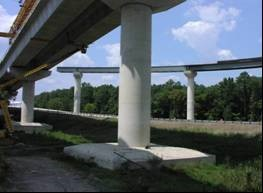
\includegraphics[width=0.7\linewidth]{mass-concrete.jpg}
  % \caption{Mass concrete; footings and columns. (Courtesy Virginia DOT)}
  \caption{大体积混凝土:立柱与基础}
  \label{fig:mass-concrete}
\end{figure}

Also, high temperatures exceeding 160°F during the first few hours following placement can lead to delayed ettringite formation (DEF) at later ages. Ettringite forms when gypsum and other sulfate compounds react with calcium aluminate in cement in the first few hours after mixing with water (Kosmatka and Wilson 2011). However, at high temperatures the normal formation of ettringite during the first few hours is impeded and DEF occurs in hardened concrete, which can crack the concrete. Heat related cracking can also occur in bridge decks that are typically not considered to be mass concrete (\cref{fig:thermal-cracks}). In this case the bridge beams restrain temperature related movement of the deck. The heat of hydration causes the deck to expand and then contract during cooling and the beams restrain the movement. To prevent the strains and resulting tensile stresses, a maximum temperature differential of 22°F between the beams and the deck is recommended for at least 24 hours following concrete placement (Babaei and Fouladgar 1997). As in the mass concrete, higher temperatures may be justified, but require detailed analysis to justify. To minimize the potential for temperature-related cracking, the amount of portland cement should be minimized, concrete delivery temperature reduced, and pozzolans and slag included in the mixture. With proper temperature management thermal cracks can be minimized and controlled.

\begin{figure}
  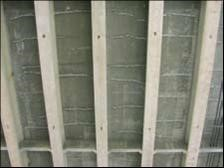
\includegraphics[width=0.6\linewidth]{thermal-cracks.jpg}
  % \caption{Thermal cracks in bridge deck. (Courtesy Virginia DOT)}
  \caption{桥面板的温度裂缝}
  \label{fig:thermal-cracks}
\end{figure}

Volumetric changes also occur due to freezing and thawing cycles and chemical (corrosion, ASR, ACR) reactions.

\subsubsection{Prevention of Distress}

\paragraph{Surface Treatments}
Surface treatments, membranes, sealers, and overlays are widely used to reduce solution infiltration. They protect the deck concrete from deterioration induced by freeze/thaw cycles, and protect the reinforcement from corrosion (Kepler et al. 2000). Currently, there are three types of waterproofing membranes used in North America: preformed sheets, liquid membranes, and built-up systems. Preformed systems can be labor intensive to install, and are vulnerable to poor workmanship at critical locations, such as curves, expansion joints, and drains. Defects and blisters have to be repaired by puncturing and patching the membrane. Liquid systems are less vulnerable to poor workmanship, and blisters and pinholes are easy to repair in self-sealing materials, but not in thermosetting materials. Built-up systems are not often used because they are generally labor intensive and expensive (Manning 1995).

To perform well, a membrane must be well bonded and undamaged, characteristics that depend on the quality of workmanship during installation. Waterproof membranes cannot stop corrosion that is already underway in existing decks, but when combined with an asphalt overlay, they can extend the service life of a deck by providing a smooth riding surface, preventing the development of potholes, and possibly slowing the rate of corrosion by limiting additional chloride contamination (Manning 1995).

Sealers can be used to protect all of the exposed concrete surfaces of the structure, including bridge decks, substructure members, and deck undersides (Zemajtis and Weyers 1996). Sealers can either be pore blockers, forming a microscopically thin (up to 2 mm) impermeable layer on the concrete surface, or they can penetrate into the concrete slightly (1.5 to 3 mm) and act as hydrophobic agents (Zemajtis and Weyers 1996). Most pore blockers are not appropriate for use on bridge decks because they do not offer good skid resistance and do not hold up under traffic wear (Sherman et al. 1993).

An important property of a sealer is its vapor transmission characteristics. Moisture within the concrete needs to be able to pass through the sealer and escape to prevent high vapor pressures from building up in the concrete during drying periods which could cause the sealer to blister and peal (Sherman et al. 1993).

\paragraph{Control of Volumetric Changes due to Moisture and Temperature}
To minimize volumetric changes due to shrinkage and temperature, low cementitious material, low water content, and low paste content are desirable. This can be achieved by using well-graded aggregates, reducing mix temperature, and the admixtures.


\paragraph{Control of Wear and Abrasion}
Traffic on bridge decks cause abrasion. Moving water also carries objects that can cause abrasion. Studded tires are very damaging to the surface of the concrete and are not permitted in some states and many other states have seasonal restrictions. Chains also have damaging effect, though, not as much as the studs. Chains are encouraged in winter in many areas and some states require chains for commercial trucks. Abrasion resistance of concrete is a function of the water cementitious material ratio (w/cm) at the surface and the aggregate quantity and quality. The Los Angeles abrasion test indicates the abrasion resistance of aggregates and in general, siliceous aggregates provide satisfactory abrasion resistance. Proper finishing and curing are also factors which influence abrasion resistance.



\paragraph{Control of Freeze/Thaw Damage}
Concrete that can become critically saturated and exposed to cycles of freezing and thawing must be properly air entrained, have sound aggregates and have the maturity to develop a compressive strength of about 4000 psi to avoid cracking and scaling (Mather 1990). Air voids must be small in size, closely spaced and uniformly distributed to ensure adequate resistance to freezing and thawing and satisfactory strength. A spacing factor less than 0.008 in. is needed for adequate protection during freezing and thawing. However, with the use of high range water reducing admixtures and low permeability concretes, higher values may be acceptable and should be verified by relevant tests such as \acrshort*{astm} C 666 Procedure A.

\paragraph{Control of Chemical Reactions}
Disruptive chemical reactions can occur in concrete that adversely affect durability. The chemical composition of the cemetitious material affects the rate of hydration and pozzolanic reaction, heat generation, and contributes to the formation of disruptive products. The fineness of the cementitious material affects the rate of reactions and water demand. At high water w/cm, permeability is increased and durability is reduced. The presence of certain chemicals in sufficient amounts in the cements contributes to the expansion. A further explanation follows.

% \subparagraph{Alkali-Aggregate Reaction (AAR)}
\subparagraph{\acrfull*{aar}}
Alkali-aggregate reactions are the reactions between the hydroxide ions in the pore fluid of concrete, usually associated with alkalis from the cement or from outside sources such as deicing salts, and the reactive constituents of the aggregates (ACI 221.1R, 1998). This reaction results in expansion and cracking.
% \subparagraph{Alkali-Silica Reaction (ASR)}
\subparagraph{\acrfull*{asr}}
A chemical reaction between aggregates containing reactive silica and the alkalis in concrete can produce an alkali-silica gel that swells when water is absorbed. The high pressures generated within the concrete lead to cracking (\cref{fig:asr}). To prevent ASR, non-reactive aggregates, or pozzolanic materials or slag, lithium nitrate, lowpermeability concrete and cements with low alkali contents are used.

\begin{figure}
  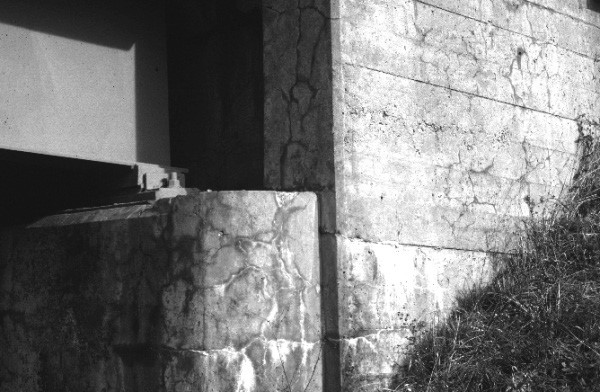
\includegraphics[width=0.6\linewidth]{asr.jpg}
  % \caption{ASR. (Courtesy Virginia DOT)}
  \caption{\acrlong*{asr}}
  \label{fig:asr}
\end{figure}

% \subparagraph{Alkali-Carbonate Reaction (ACR)}
\subparagraph{\acrfull*{acr}}
Some argillaceous, dolomitic aggregates can react with alkalis, causing the aggregates to expand. \cref{fig:acr} shows a joint closing due to ACR expansion. A common prevention for ACR is to avoid using reactive aggregate or to dilute the aggregate by blending with non-reactive aggregate.

\begin{figure}
  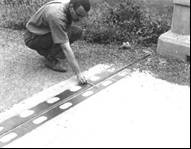
\includegraphics[width=0.6\linewidth]{acr.jpg}
  % \caption{Closing of joints due to ACR. (Courtesy Virginia DOT)}
  \caption{由\acrlong*{acr}引起的接缝闭合}
  \label{fig:acr}
\end{figure}

\subparagraph{Carbonation}
Carbon dioxide produced by plants penetrates concrete and reacts with the hydroxides, such as calcium hydroxide, to form carbonates. In this carbonation process the pH is reduced to less than nine, influences the protective layer over the steel (Neville 1995).

\subparagraph{Chlorides}
Chlorides which penetrate the concrete and reach the steel surface destroy the protective oxide layer making reinforcement prone to corrosion. Without the protective layer, steel will corrode rapidly in the presence of water and oxygen. The corrosion of steel is accompanied by expansive pressures, which lead to cracking (\cref{fig:chlorides-corrosion}). To stabilize the passive oxide layer on the reinforcement, corrosion inhibiting admixtures can be used or, viscosity modifying admixtures can be added to improve the stability of the mix.

\begin{figure}
  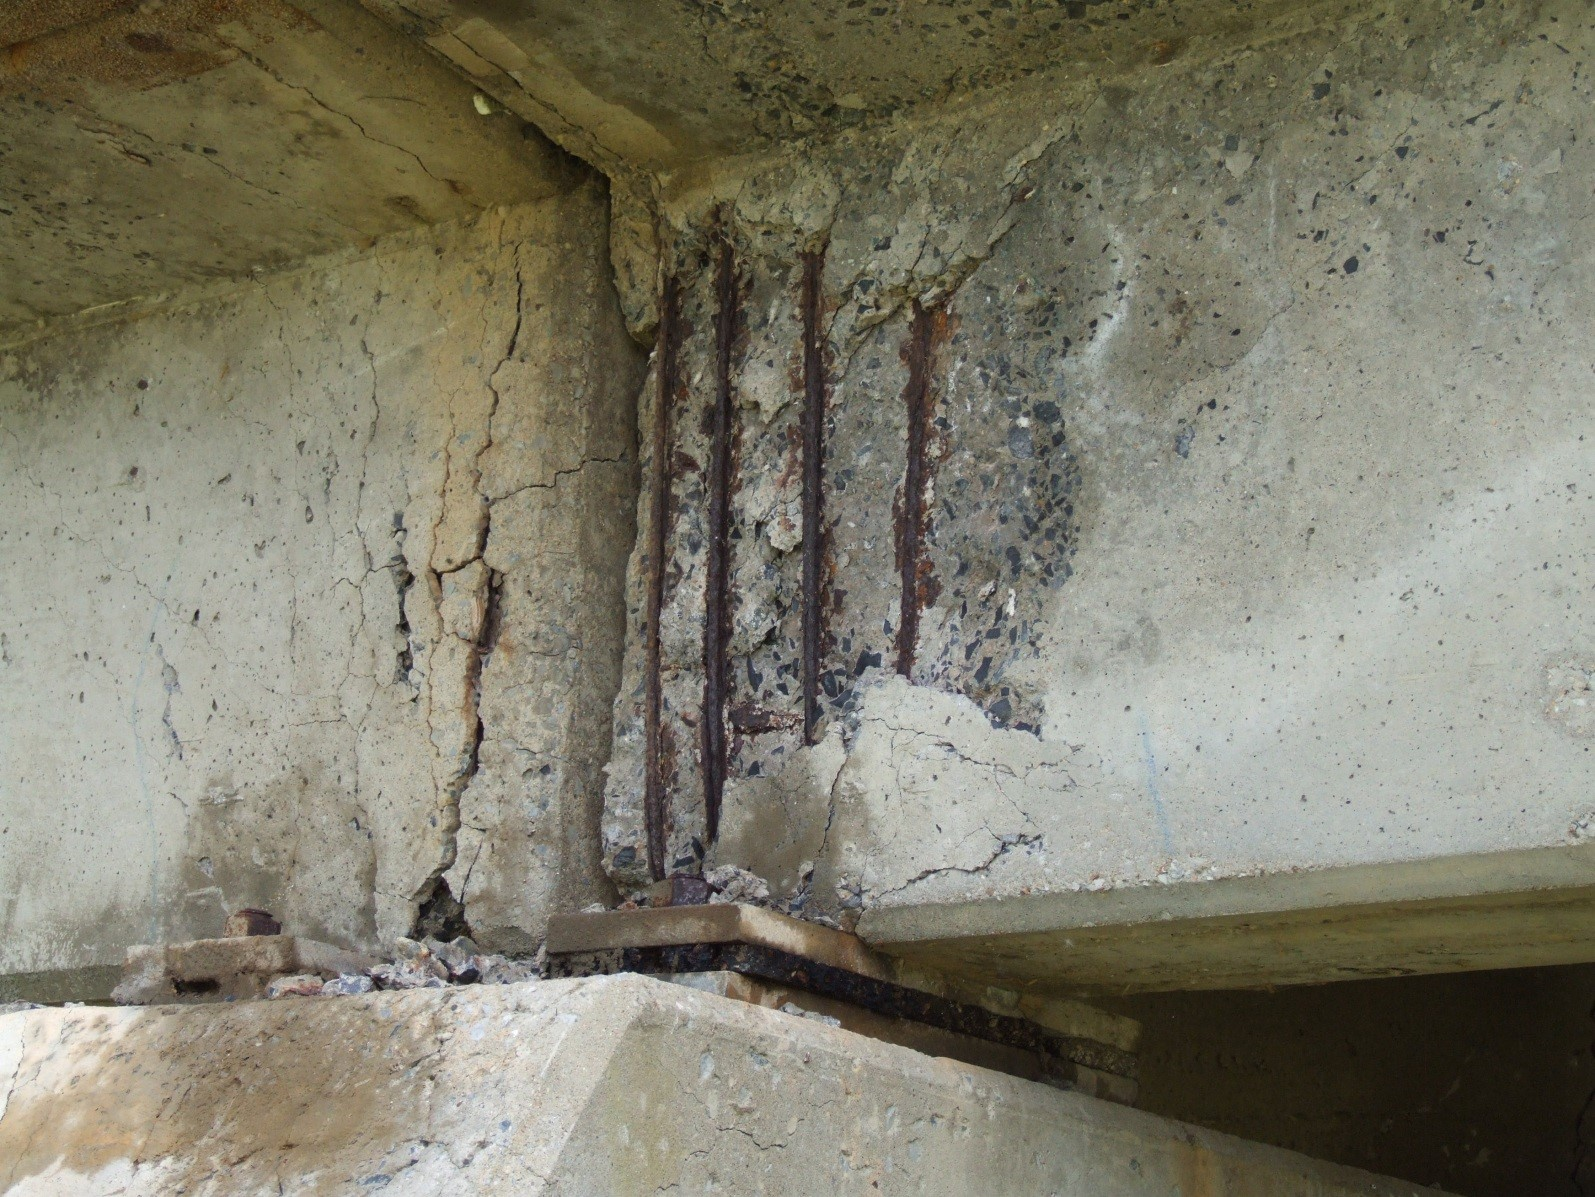
\includegraphics[width=0.6\linewidth]{chlorides-corrosion.jpg}
  % \caption{Corrosion. (Courtesy Virginia DOT)}
  \caption{腐蚀}
  \label{fig:chlorides-corrosion}
\end{figure}

\subparagraph{Sulfates}
Sulfates react with the \ce{Ca(OH)2} and the calcium aluminate hydrates causing expansive reactions that can affect the cement paste (Neville 1995). \cref{fig:sulfate} displays the loss of material due to sulfate attack. To increase the resistance of concrete to sulfate attack a low C3A, tricalcium aluminate, content, low quantities of \ce{Ca(OH)2}, calcium hydroxide (lime), in the cement paste, and low permeability concrete is needed. These results can be obtained by using sulfate resistant cements and use of pozzolans.

\begin{figure}
  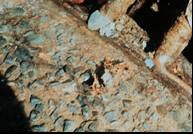
\includegraphics[width=0.6\linewidth]{sulfate.jpg}
  % \caption{Sulfate attack. (Courtesy Virginia DOT)}
  \caption{硫酸盐侵袭}
  \label{fig:sulfate}
\end{figure}


\subparagraph{Acids}
Pollutants cause acid rain that can cause deterioration (Neville 1995). In damp conditions, \ce{SO2}, \ce{CO2}, \ce{SO3} and other acid forms that are present in the atmosphere may attack concrete by dissolving in water and removing parts of the cement paste. These acids will leave a soft and mushy mass behind (Eglinton 1975). To minimize acid attack, low-permeability concrete and barrier coatings may be used. A barrier material separates the concrete surface from
the environment.


\subparagraph{Salts}
Chloride bearing deicing chemicals initiate and accelerate corrosion. Magnesium salts are very damaging to concrete causing crumbling (Lee et al. 2000). Calcium magnesium acetate has been suggested to prevent corrosion but was found to be very damaging to concrete. Deicing chemicals can also aggravate freeze/thaw deterioration. Osmotic pressure occurs since moisture tends to move towards zones with higher salt concentrations. In addition the salts increase the rate of cooling causing an increase in the potential for freeze/thaw deterioration at the concrete surface. Proper air entrainment and maturity are also needed to provide the necessary protection.


\paragraph{Functional Considerations}
Functional considerations include vibrations, impact, concrete consolidation, concrete curing, and concrete placement.

\subparagraph{Vibrations}
Vibration of fresh concrete using vibrators may cause loss of air in mixtures with a high sand content and could result in freeze/thaw damage. In these mixtures, the frequency and duration of vibration should be reduced to prevent segregation (loss of stability) and loss of air. A recommended practice is to prepare mixtures with a large amount of coarse aggregate content. However, in some regions where D-cracking (\cref{fig:d-cracking}) is an issue the size and amount of coarse aggregate is reduced which leads to mixtures with an excessive sand content. In D-cracking, the aggregate has a pore structure that hinders the expulsion of water from the aggregate pores during freezing resulting in the cracking of the aggregate and concrete.

\begin{figure}
  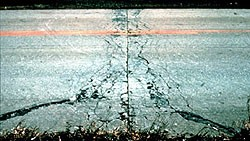
\includegraphics[width=0.6\linewidth]{d-cracking.jpg}
  % \caption{D-cracking. (Courtesy of PCA)}
  \caption{D-cracking. (Courtesy of PCA)}
  \label{fig:d-cracking}
\end{figure}

Concrete can exhibit fatigue behavior when subjected to cyclic loading of a given level, below its short-term static strength, and will eventually fail.

\subparagraph{Impact}
Concrete can be subjected to extreme loads due to impact of falling rocks, snow avalanches, landslides, or vehicle crashes. The impact resistance is related to the compressive strength and aggregate type (Kosmatka and Wilson 2011). Fiber reinforced concretes are used to minimize the effect of impact in certain applications.


\subparagraph{Concrete Consolidation}
Proper consolidation ensures that undesirable entrapped air voids are eliminated. Voids in concrete reduce strength and when interconnected or in large amounts can increase permeability. Currently, workable concretes are made using water reducing admixtures. It is also possible to make stable concretes that have high flow rates and are self consolidating.

\subparagraph{Concrete Curing}

Curing ensures that reactions occur and volumetric changes are minimized. Curing should continue until a certain level of the desired properties is achieved. Concrete should stay wet during the curing period and the temperature should be managed to eliminate large differentials. ACI 308R provides recommendations for adequate curing. ACI 305R and ACI 306R provide information on curing of concrete in hot and cold weather respectively.

\subparagraph{Concrete Placement}
Concrete should be placed without causing segregation and loss of moisture. Forms should be adequately set, clean, tight, and adequately braced. Forms should be oiled or treated with a form-release agent. Reinforcing steel should be clean and free of rust or mill scale. In cold weather, concrete should not be placed in contact with metal forms and embedments, such as steel structural members or reinforcement, that can freeze the concrete (ACI 306R, 2010). If the frozen concrete does not thaw before the bulk of the concrete sets, bond may be significantly reduced, and concrete quality adjacent to cold metal would be poor. Ideally, the adjacent metal should be heated to the temperature of the concrete immediately before concrete placement (ACI 306R, 2010). Concrete should be deposited continuously and as near as possible to its final position without objectionable segregation (Kosmatka and Wilson 2011). Concrete should be deposited in areas free of standing water. However, in some applications such as drilled shafts standing water may be present. In such applications, concrete should be placed in a manner that it displaces the water ahead of the concrete without mixing with the concrete. Pumps and tremies with ends buried in the fresh concrete can be used to maintain a seal below the rising surface. Pumps are widely used to place concrete in bridge structures. Care should be exercised in delivering with the pump since free fall within the pump hose can result in loss of slump and air.


% \subsection{Protection of Reinforcing Steel against Corrosion}
\subsection{钢筋防腐蚀保护}
\label{subsec:protection-reinforcing-steel}
% Methods for protecting reinforcing steel elements from corrosion include the use of corrosion-resistant reinforcing steel and the use of non-intrinsic protection of the reinforcement (such as admixtures, cathodic protection systems, and electrochemical chloride extraction techniques) as described in the following. \cref{chp:corrosion-of-steel-rc-bridge} also covers the cathodic protection system and electrochemical chloride extraction in additional detail.
保护钢筋免受腐蚀的方法包括使用耐腐蚀钢筋和使用钢筋的非内在保护(如外加剂、阴极保护系统和电化学氯化物萃取技术),如下所述。\cref{chp:corrosion-of-steel-rc-bridge}还详细介绍了阴极保护系统和电化学氯化物提取。

% \subsubsection{Corrosion-Resistant Reinforcement}
\subsubsection{耐腐蚀钢筋}
% Corrosion-resistant reinforcement allows chlorides to penetrate around the reinforcement without causing significant damage to the reinforcing steel. These systems include epoxy-coated reinforcement, galvanized reinforcement, titanium reinforcement, stainless steel reinforcement, stainless steel clad reinforcement, nickel-clad reinforcement, and copper-clad reinforcement. Following is a description of the protection expected from these materials.
耐腐蚀钢筋允许氯离子渗透到钢筋材料周围,而不会对钢筋造成重大损坏。这些系统包括环氧涂层钢筋、镀锌钢筋、钛合金钢筋、不锈钢钢筋、不锈钢覆层钢筋、镍覆层钢筋和铜覆层钢筋。以下是对这些材料所期望的保护的描述。

% \paragraph{Epoxy-Coated Reinforcement (ECR)}
\paragraph{\acrfull*{ecr}}
% Tests have shown that the diffusion rates of oxygen and chloride ions through a quality coating of adequate thickness 177 μm (7 mils) are extremely low, even in severe exposure conditions (Clifton et al. 1974; Pike 1973). However, epoxy-based coatings are not impermeable to water (Lee and Neville 1967).
试验表明,即使在恶劣的暴露条件下,氧和氯离子通过具有足够厚度(\qty{177}{\micro m})优质涂层的扩散速率极低(Clifton 等人,1974 年;派克1973)。然而,环氧基涂料并非不透水(Lee and Neville 1967)。

ECR extends service life; however, experience in Florida and Virginia has shown that epoxy coating on ECR naturally degrades in the highly alkaline moist environment within concrete (Weyers et al. 2006). The estimated service life benefit of ECR may be as little as 3 to 5 years (Weyers et al. 2006). Today, structures are designed for service lives of 75 or 100 years, but the long-term protection provided by ECR is uncertain (Hartt et al. 2009). The improvements observed by some and attributed to ECR have coincided with other improvements such as reduced w/cm and increased cover.

\paragraph{Galvanized Reinforcement}
Zinc coatings have a higher chloride (\ce{Cl-}) corrosion threshold (2 to 4 times) than that of uncoated steel, significantly extending the time until corrosion initiation (Yeomans 2004). Once corrosion of the zinc does occur,
the properties of the corrosion products and their ability to migrate into the concrete matrix reduces stress generation in the surrounding concrete, further extending the life of the reinforced concrete structure.

One major drawback in the use of galvanized bar is the uncertainty that exists due to the effect of galvanizing on the brittleness of bars of different composition and with different degrees of work hardening. Some individuals believe it is preferable to bend cold-worked bars after galvanizing, even at the risk of damaging the zinc coating. It is generally easier and more economical to galvanize straight lengths of reinforcing bars completing all fabrication after galvanizing.

\paragraph{Titanium Reinforcing Bars}
McDonald et al. (1995) found the corrosion rate of titanium bars to be 14,000-times less than that of black steel in a neutral solution and 135-times less than that of black steel in a high pH salt solution. The study estimated that titanium bars would extend the time-to-corrosion related cracking of concrete by about 130 times.

\paragraph{Stainless Steel Reinforcement}
Chloride threshold values for stainless steel have been reported to be at least 10.4-times greater than for carbon steel (Cleme\~{n}a 2003).

Solid stainless steel is preferred over stainless steel-clad carbon steel in Europe because the process of fusing the two types of metal together is not considered to be cost-effective. Another advantage of solid stainless steel bars is that they can be shipped, handled and bent without fear of damage to the coating (Smith and Tullmin 1999). In addition, the ends do not have to be coated after cutting (Russell 2004). \cref{fig:stainless-reinforcement} shows disbondment after cutting.

\begin{figure}
  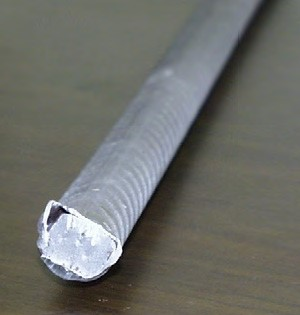
\includegraphics[width=0.6\linewidth]{stainless-reinforcement.jpg}
  % \caption{Stainless steel-clad reinforcement (disbondment after cutting). (Deshpande et al. 2000)}
  \caption{Stainless steel-clad reinforcement (disbondment after cutting). (Deshpande et al. 2000)}
  \label{fig:stainless-reinforcement}
\end{figure}

Stainless steel is often used in areas in which sufficient cover cannot be obtained or at construction joints and critical gaps between columns and decks. Because of stainless steel cost, estimated to be four to six times more than black bar, it is not expected to be a standard for all reinforcement. Darwin et al. (2002) compared the costs of different types of reinforcement in a thick deck and reported that the initial cost of deck area for stainless steel was approximately 1.4-times more expensive than conventional reinforcement. However, based on total costs over 75 years, the stainless steel reinforcement was more economical.

The FHWA study Corrosion Evaluation of Epoxy-Coated, Metallic-Clad, and Solid Metallic Reinforcing Bars in Concrete (McDonald et al. 1998) examined two types of solid stainless steel in concrete exposure specimens, \acrshort*{astm} A955 Types 304 and 316. The results show that the lowest corrosion rates for Type 304 bars were obtained when the stainless steel was used in both bridge deck mats. Cracks in the concrete did not appear to affect the performance of the stainless steel bars. Half of the bars from specimens that contained black steel in the bottom mat exhibited moderate to high corrosion currents and had red rust on them. When the stainless steel bars were used in both mats, the specimens did not exhibit any signs of chloride-induced corrosion, even when the slabs were pre-cracked. Both conditions (cracked and uncracked concrete) had about 1,500-times lower corrosion rates than black steel specimens. Corrosion currents on bars with black bottom mats were 20- and 700-times lower than for black steel specimens, for bent and straight bars, respectively.

All of the specimens containing Type 316 solid stainless steel showed good corrosion performance. There was no distinguishable difference between pre-cracked and uncracked slabs or between slabs with a black steel cathode or a stainless steel cathode. Measured corrosion for all conditions was about 800-times lower than that of the black steel specimens. During visual inspection of the slabs, only one of the bars exhibited corrosion and it was considered to be minor.


\paragraph{Nickel-Clad Reinforcing Bars}
Nickel claddings for steel reinforcing bars were first used in the late 1960s. The corrosion resistance of nickel in alkaline chloride solutions is high, and although steel is less noble than nickel, the corrosion of the underlying steel is not substantially accelerated if breaks occur in the barrier (Tripler et al. 1966). Although research has been promising so far, steel bars with a nickel cladding of ample thickness to prevent corrosion damage are relatively expensive (Virmani and Clemeña 1998).


\paragraph{Copper-Clad Reinforcement}
Copper-clad reinforcing bars were compared to black steel in concrete with and without calcium nitrite corrosion inhibitors and to non-specification epoxy-coated bars. The non-specification bars had been coated for an earlier study and stored outdoors for over two years; the bars used in the study all contained more than 25 holidays per foot and failed the \acrshort*{astm} bend test. Visible damage to the epoxy-coatings was estimated at less than 0.05\% of the surface area. The copper-clad bars were not discussed in the FHWA report, but the results were published by McDonald et al. (1996). These results indicate that the copper-clad bars, with a coating thickness of about 0.5 mm (0.02 in.), exhibited much better corrosion resistance than the other types of reinforcement in the study, even the black steel with calcium nitrite corrosion inhibitor. Slabs containing copper-clad bars in the top mat only and in both mats were still in good condition after 13 years of outdoor exposure with no visible cracks. The average total chloride contents in the slabs were 8.50 to 10.32 kg/m3 (14.33 to 17.40 lb/yd3), which is well above the corrosion threshold level of steel. Copper is more noble than steel and could lead to corrosion of steel exposed in defect areas.

Tests up to this time (2012) have shown excellent corrosion resistance for copper-clad reinforcing bars in concrete and they could prove to be cost effective. However, before copper-clad reinforcement can be put to use in any structures, research needs to be performed on the structural effect of the retardation of cement hydration that is caused by these bars (McDonald et al. 1996; Virmani and Clemeña 1998).


\subsubsection{Non-Intrinsic Corrosion Protection of Reinforcement}

\paragraph{Admixtures for Corrosion Protection}
Chemical admixtures that are added to concrete during batching to protect against corrosion of embedded steel reinforcement due to chlorides are available. There are two main types: corrosion inhibitors and physical-barrier admixtures. Some corrosion inhibitors also act as physical barrier admixtures (ACI 222.3R, 2003).

Corrosion inhibitors, although known for many years, are only now beginning to be actively marketed as a preventative treatment in a concrete repair program (Macdonald 2003). Calcium-nitrite admixtures are the most researched inorganic inhibitor and the most widely used (Berke and Rosenberg 1989). Inhibitors do not create a physical barrier to chloride ion ingress. Rather, they modify the steel surface, either electrochemically (anodic, cathodic, mixed-inhibitor) or chemically (chemical barrier) to inhibit chloride-induced corrosion above the accepted chloride-corrosion threshold level. They are added to the concrete at the time of batching (ACI 201.2R, 2008). Calcium nitrite is also an accelerating admixture. If the accelerating effect is undesirable, a retarding admixture can be added.

There are also admixtures with organic compounds which protect steel from chloride-induced corrosion. They include alkanolamines and an aqueous mixture of amines and fatty-acid esters (Nmai et al. 1992; Nmai and Krauss 1994). They are claimed to both reduce ingress of chlorides (physical barrier) and enhance the passivating layer on the steel surface (corrosion inhibitor). Other similar amine products are claimed to migrate through concrete in the vapor phase to provide protection to embedded steel. Corrosion inhibitors are attractive from a conservation point of view as they are almost invisible on application, although their long-term visual effect is unknown (Macdonald 2003).

Physical-barrier admixtures reduce the rate of ingress of corrosive agents (chlorides, oxygen, and water) into the concrete. These admixtures belong to one of two groups. One group comprises waterproofing and damp-proofing compounds. The second group consists of agents that create an organic film around the reinforcing steel, supplementing the passivating layer. They typically contain bitumen, silicates and water-based organic admixtures consisting of fatty acids, such as oleic acid; stearic acid; salts of calcium oleate; and esters, such as butyloleate (ACI 222R 2001). A liquid admixture containing a silicate copolymer in the form of a complex, inorganic, alkaline earth may also be effective in reducing the permeability of concrete and providing protection against corrosion of reinforcing steel (Miller 1995).



\paragraph{Cathodic Protection}
Cathodic protection can effectively stop corrosion in contaminated reinforced concrete structures and can reduce the concentration of chloride ions at the steel surface of protected reinforcement (Kepler et al. 2000).

An advantage of using cathodic protection as a repair method for reinforced concrete bridges is that only spalls and detached concrete need to be repaired. Chloride-contaminated concrete that is still sound can remain in place because the cathodic protection system will prevent further corrosion and will, in fact, reduce the concentration of chloride ions adjacent to the protected reinforcing bars. This can significantly reduce repair costs (Polder 1998).

Both impressed current and sacrificial anode, or galvanic systems, have been used successfully on bridges in the United States. Impressed current systems are used most often on bridge decks, but there are some impressed current anodes that can be used on bridge substructure members as well. Historically, the use of galvanic anodes has been generally limited to substructure members (Kepler et al. 2000).

The wide use of cathodic protection has been hampered by the high cost and the maintenance of the power source or the protective material.

\paragraph{Electrochemical Chloride Extraction (ECE)}
Electrochemical chloride extraction is applied to concrete structures containing reinforcement in order to extract chlorides from the concrete. ECE involves the application of current (1A/m2 of steel) typically over a 4- to 8-week period. The steel acts as a cathode and is connected to the negative pole of the power source. The anode, which is either steel or a titanium mesh, is temporarily placed on the concrete cover and is connected to the positive pole of the power source. The electrolyte is placed on the concrete cover and allows the current flow. It is important to provide a buffer in order to keep a constant pH if titanium mesh is used. Due to the electric field, the negative ions, like chlorides, migrate from the rebar to the concrete cover. The electrochemical chloride extraction, using a current density of 1A/m2 of steel for eight weeks (total charge 1344 A.h/m2), removes about 40\% of the initial free chloride on the average concrete

With ECE, the possibility of initiating the alkali-silica reaction as a side effect exists, as alkali metal ions are rearranged and hydroxyl ions are generated at the reinforcement. The pH necessary to initiate alkali-silica reaction is not known, but it can be assumed that if a structure is suffering from corrosion due to saltwater ingress, the concentration of sodium ions may be above the threshold for sustaining alkali-silica reaction (Kepler et al. 2000).  Studies have indicated that the alkali-silica reaction can be mitigated by lithium (Velivasakis et al. 1997).
\paragraph{Other Protective Methods}

Other protective methods include the use of drainage design, and stay-in-place metal forms. Posttensioning of members would also eliminate the formation of cracks.

% \section{Factors Influencing Service Life Using Fault Tree}
\section{使用\glsentrytext{faulttree}分析影响\glsentrytext{servicelife}的因素}
\label{sec:factor-influence-fault-tree}
\subsection{Service Life of Concrete}
Concrete deterioration is caused by deficiencies in one or more factors listed as materials, design, and workmanship; the effect of external factors; and the occurrence of cracks. These factors are shown in the main fault tree (\cref{fig:faulttree-concrete-reduced-main}) and are explained in additional detail in the fault trees for each factor, \cref{fig:fault-tree-material,fig:faulttree-design,fig:fault-tree-workmanship,fig:fault-tree-load,fig:fault-tree-environment,fig:fault-tree-cracking}.

\begin{figure}
  % \includegraphics{fig:faulttree-concrete-reduced-main.pdf}
  % \caption{Concrete reduced service life main fault tree.}
  \caption{Concrete reduced service life main fault tree.}
  \label{fig:faulttree-concrete-reduced-main}
\end{figure}


\subsubsection{Material}
Material-related factors are shown in \cref{fig:fault-tree-material}. They include the ingredients of the concrete—the cementitious material, aggregates, water, admixtures, and fibers. The water-cementitious materials ratio (w/cm) is also included in this module. The information on materials is given in \cref{sec:material-types} under description of material types. The cementitious materials have different chemical and physical properties that affect the hydration reaction, harmful chemical reactions, and volumetric changes that relates to the durability of concrete. The type, quality, grading, and texture of the aggregates affect the water content and durability. Aggregates may cause D-cracking, ASR, and ACR; therefore, precautions need to be taken in order to inhibit such occurrences. Water, whether it is potable or recycled, may have some excessive impurities that may cause durability problems due to expansive chemical reactions and increased w/cm. Small solid particles in water have large surface area; they increase the water demand and the w/cm if the cement content is kept the same. Admixtures help in achieving workable, low w/cm, and low permeability concretes leading to improved durability. Fibers are used to control cracking.

\begin{figure}
  % \includegraphics[width=\linewidth]{graphic-file}
  % \caption{Materials fault tree.}
  \caption{材料\gls*{faulttree}}
  \label{fig:fault-tree-material}
\end{figure}

\subsubsection{Design}
Design of the structure through the selection of the geometry, detailing, and flexibility affects the performance of the concrete. The design fault tree is shown in \cref{fig:faulttree-design}. In the geometry, the cover depth over the reinforcement has a large influence on the salt intrusion to the level of steel. Thicker decks provide more rigidity and less cracking potential. Long-span length causes more flexibility, increasing the possibility of cracking.

Design details which minimize saturation with water would lead to improved durability. Eliminating joints is desirable since joints cause leakage problems.

\begin{figure}
  % \includegraphics[width=\linewidth]{faulttree-design.pdf}
  % \caption{Design fault tree}
  \caption{设计\gls*{faulttree}}
  \label{fig:faulttree-design}
\end{figure}

\subsubsection{Workmanship}
Workmanship is important in achieving the desired durability; the materials have to be fabricated properly under adequate inspection to achieve the desired performance. Frequent maintenance to correct deficiencies is also needed to eliminate premature failure of the elements. Fabrication of components includes mixing, consolidation, finishing, and curing as shown in the workmanship fault tree, \cref{fig:fault-tree-workmanship}.

\begin{figure}
  % \includegraphics[width=\linewidth]{graphic-file}
  % \caption{Workmanship fault tree.}
  \caption{Workmanship fault tree.}
  \label{fig:fault-tree-workmanship}
\end{figure}

The concrete mixer should be in good working order, the capacity given by the manufacturer should not be exceeded, and enough mixing time at the specified mixing rate should be maintained. Following the proper mixing guidelines will ensure a uniform consistent concrete mixture. Consolidation, which is achieved by proper internal or external vibration, eliminates the large air voids that adversely affect the strength and durability of concrete.

Bridge decks require minimal finishing operations. The vibratory screed with proper speed, vibration, and set-up of the auger and the roller, can provide adequate vibration if the workability of the concrete is adequate. The sides and ends that the vibratory screed cannot reach are finished by hand. Extra hand finishing is detrimental and may delay the curing operation and cause loss of entrained air voids near the top surface. Curing is essential for the continuation of the hydration reactions and the control of cracking due to volumetric changes. The best curing process is a water cure that enables moisture retention and temperature management. Curing compounds are also used to maintain the satisfactory moisture and temperature. Virginia DOT uses curing compounds after a seven-day wet curing of decks.


\subsubsection{External Factors}
External factors that affect the service life of concrete are loads and the environment. Loads are illustrated in \cref{fig:fault-tree-load}, and the environment in \cref{fig:fault-tree-environment}.

\paragraph{Loads}
Loads can be traffic-induced, age-dependent, or system-dependent. Traffic-induced loads are a result of the vehicle loads and the frequency of traffic imparting fatigue stresses, overloads due to unexpected high loads. The adverse effect of loads are wide and frequent cracks that facilitate the intrusion of harmful solutions. The duration of loading has to be considered, as loads can be instantaneous or time-dependent. Time-dependent loads cause additional distress and result in additional cracks. System-dependent loads are a result of moisture and temperature variation and the available restraint. When restrained, the deformations lead to stresses that can exceed the strength of the material leading to cracking. When cement reacts with water, an exothermic reaction takes place, temperature rises and heat is given off, and concrete expands. As the reaction slows, cooling takes place and thermal contraction occurs subjecting the restrained concrete to tensile stresses. When the stresses exceed the strength of the material, cracks occur. This thermal effect is more pronounced in mass concrete since the dissipation of heat is difficult in a large mass. High heat can also result in delayed ettringite reaction that can cause cracks in hardened concrete. In hot weather, thermal effects can be detrimental; however, in a cold environment, the heat of hydration can provide the favorable temperature needed for the hydration reactions.

\begin{figure}
  % \includegraphics[width=\linewidth]{graphic-file}
  \caption{Load fault tree.}
  \label{fig:fault-tree-load} 
\end{figure}

\paragraph{Environment}
Environment can provoke damage in structures caused by physical and/or chemical factors. The physical factors are the result of freezing and thawing of critically saturated concrete, scaling of surfaces due to salt concentrations or excessive wear, seismic activity, settlement, or volumetric changes due to moisture and temperature variation, or stresses due to wind velocity. Chemical factors involve corrosion; carbonation, which reduces pH and makes steel vulnerable to corrosion; sulfate attack; or expansion due to alkali-aggregate or alkali silica reactions.

\begin{figure}
  % \includegraphics[width=\linewidth]{graphic-file}
  \caption{Environment fault tree.}
  \label{fig:fault-tree-environment} 
\end{figure}

\paragraph{Cracking}
Cracking of concrete can cause serious and costly damage to concrete structures. The cracking fault tree is shown in \cref{fig:fault-tree-cracking}. The factors affecting cracking can be due to design, materials, and/or construction. In the case of design, the factors of interest include the restraint, span type, deck thickness, girder type, or the steel alignment and location. When concrete is restrained, deformations result in stresses. Flexible structures and low rigidity lead to additional cracks. For example, decks on steel beams exhibit additional cracking compared to decks on rigid concrete beams. High modulus and low creep that can be beneficial in reducing prestress losses and deflections in beams, can lead to additional cracking in decks. High modulus leads to brittle structures and low creep does not enable relaxation that reduces stresses. It can be expected that low water-cementitious material ratios, high paste contents, and high heat of hydration can cause additional cracking. Concretes with low w/cm are brittle and more sensitive to curing. Concretes with high water, cement, and paste content exhibit additional shrinkage and additional temperature rise During construction and afterwards, the weather conditions, curing, time of setting, consolidation, and curing sequence and length affect the cracking pattern and severity.

\begin{figure}
  % \includegraphics[width=\linewidth]{graphic-file}
  \caption{Cracking fault tree.}
  \label{fig:fault-tree-cracking} 
\end{figure}


\subsection{Service Life of Reinforcement}
Reduced service life of reinforcement can be attributed to three causes: load-induced, man-made or natural hazards; causes resulting from production defects in construction processes and/or design details; or operational procedures. These deficiencies are illustrated in the main fault tree shown in \cref{fig:fault-tree-reduced-main}.

\begin{figure}
  % \includegraphics[width=\linewidth]{graphic-file}
  \caption{Reduced service life main fault tree.}
  \label{fig:fault-tree-reduced-main} 
\end{figure}

\subsubsection{Load-induced}
Load-induced bridge deck deterioration can be attributed to fatigue, strength and brittleness, or thermal
incompatibility. These load-induced factors are introduced in the fault tree provided in \cref{fig:fault-tree-load-induced}.

\begin{figure}
  % \includegraphics[width=\linewidth]{graphic-file}
  \caption{Load-induced deficiency fault tree.}
  \label{fig:fault-tree-load-induced} 
\end{figure}

Fatigue is caused by the repetition of applied loads that result in a degradation of the strength resistance of the reinforcement. Information on reinforcement material is summarized in \cref{subsec:reinforcement-material}. Corrosion-resistant reinforcement (CRR) has fatigue properties similar to that of carbon steel reinforcement when tested in the atmosphere. However, in a corrosive environment, CRR performs better than the carbon steel since carbon steel is expected to corrode, lose material area, and develop corrosion pits. The fatigue limit is related to the tensile strength of the steel, hence CRR with increased strength has increased fatigue limit.

\paragraph{Strength and Brittleness}
Strength and brittleness affect cracking and failure. In general, CRR has higher tensile strength and ductility than the carbon steels. Cold-formed austenitic reinforcement has a combination of high strength and good ductility; a yield stress level of 70 ksi or higher and elongation at maximum force higher than 15\% is achieved (Bourgin et al. 2006). Duplex grades exhibit strengths exceeding 70 ksi in hot-rolled and 90 ksi in cold-rolled bars. At the higher strengths, ductility is at least as good as the carbon steels.

\paragraph{Thermal Compatibility}
\paragraph{热适应性}
% Thermal compatibility affects cracking potential. Temperature changes in a material result in deformations that can cause significant stress when restrained by the surrounding material. However, in reinforced concrete the carbon steel and concrete have similar coefficients of thermal expansion leading to negligible stresses due to temperature changes in the structure. Carbon steels have a coefficient of thermal expansion (CTE) of about 5.5 x 106/ºF; CRR with austenitic steels have a CTE of approximately 8.9 x 106/ºF; and the austenitic-ferritic duplex steels have a CTE of about 7.2 x 106/ºF (Markeset et al. 2006). There has been no reported problem due to these differences.
热适应性会影响开裂可能性。材料中的温度变化会导致变形,当受到周围材料的约束时,变形会导致显著的应力。然而,在钢筋混凝土中,碳钢和混凝土具有相似的热膨胀系数,导致由于结构中的温度变化而产生的应力可以忽略不计。 碳钢的热膨胀系数 (CTE) 约为 5.5 x 106/ºF; 奥氏体钢的 CRR 的 CTE 约为 8.9 x 106/ºF; 奥氏体-铁素体双相钢的 CTE 约为 7.2 x 106/ºF(Marketet 等人,2006 年)。 由于这些差异,尚未报告任何问题。

% \subsubsection{Natural or Man-Made Hazards}
\subsubsection{自然或人为危害}
% Natural or man-made hazards include effects from areas with adverse thermal climate, coastal climates and chemical climates, and fire. These natural and man-made hazards are introduced in the fault tree provided in \cref{fig:fault-tree-natural-manmade}.
自然或人为危害包括不利热气候、沿海气候和化学气候以及火灾地区的影响。 这些自然和人为的危害在 \cref{fig:fault-tree-natural-manmade} 中提供的\gls*{faulttree}中进行了介绍。

% \paragraph{Thermal Climate}
\paragraph{热气候}
% Thermal climate affects the corrosion activity. In cold climates, chloride-bearing deicing salts are commonly used to prevent ice buildup on roads. Chlorides destroy the protective iron oxide layer over the carbon steels exposing the reinforcement to corrosion. Corrosion of prestressing steel is generally a greater concern than corrosion of nonprestressed reinforcement because of the possibility that corrosion may cause a local reduction in cross section and failure of the prestressing steel\cite{aci2001p}. The typical higher stresses in the prestressing steel also render it more vulnerable to stress-corrosion cracking and to corrosion fatigue. Because of the potentially greater vulnerability and the consequences of corrosion of prestressing steel, chloride limits for prestressed concrete are lower than those for reinforced concrete \cite{aci2001p}.
热气候影响腐蚀活动。 在寒冷气候下,含氯化物的除冰盐通常用于防止道路结冰。氯化物会破坏碳钢上的氧化铁保护层,使钢筋暴露在腐蚀之下。预应力钢筋的腐蚀通常比非预应力钢筋的腐蚀更受关注,因为腐蚀可能导致横截面局部减小和预应力钢筋失效\cite{aci2001p}。 预应力钢中典型的较高应力也使其更容易发生应力腐蚀开裂和腐蚀疲劳。 由于预应力钢材可能存在更大的脆弱性和腐蚀后果,因此预应力混凝土的氯化物限值低于钢筋混凝土 \cite{aci2001p}。

% Corrosion rate is dependent on the temperature, humidity, and chloride content. An increase in temperature in dry environments results in reduced corrosion activity and an increase in expected life (Lopez et al. 1993). However, in environments with high humidity, increasing temperatures result in increased corrosion activity leading to reduced expected life.
腐蚀速率取决于温度、湿度和氯化物含量。 干燥环境中温度的升高会导致腐蚀活动减少和预期寿命增加(Lopez 等人,1993 年)。 然而,在高湿度环境中,温度升高会导致腐蚀活动增加,从而导致预期寿命缩短。

% Low temperature, cryogenic applications, can cause brittle failure. Carbon steel reinforcement exhibits brittle behavior below 0°F when exposed to sudden loading and seismic actions. Austenitic stainless steels do not present such a transition; therefore, can be used in cryogenic applications; their toughness remains very high at temperatures as low as -320°F. Duplex stainless steel may not be used below -60°F (Markeset et al. 2006).
低温、低温应用会导致脆性失效。 当暴露于突然加载和地震作用时,碳钢钢筋在 \qty{-17.8}{\celsius} 以下表现出脆性行为。 奥氏体不锈钢不存在这种转变; 因此,可用于低温应用; 它们的韧性在低至 \qty{-195}{\celsius} 的温度下仍然非常高。 双相不锈钢不得在 \qty{-50}{\celsius} 以下使用(Marketset 等人,2006 年)。

% \paragraph{Coastal Climate}
\paragraph{沿海气候}
% Coastal climate introduces salt spray and high humidity, and salt and moisture accelerates the corrosion rate. Salt spray in coastal climates provides high chloride buildup that can destroy the protective iron oxide coating over the steel reinforcement.
沿海气候引入盐雾和高湿度,盐和水分加速腐蚀速度。沿海气候下的盐雾会产生大量氯化物,会破坏钢筋上的保护性氧化铁涂层。

% Humidity affects corrosion activity. In the absence of chloride ions, little corrosion activity takes place when the relative humidity is under 60\% (Jung et al. 2003). The corrosion activity increases as the RH is increased up to a fully saturated state (>95\% relative humidity) and then begins to decrease again. When concrete is fully saturated, the corrosion rate is reduced because the oxygen level in the concrete pores is too low (Qian et al. 2002). When chlorides are present at relative humidity below 60\%, corrosion activity may still develop.
湿度影响腐蚀活动。 在没有氯离子的情况下,当相对湿度低于 60\% 时,几乎不会发生腐蚀活动 (Jung et al. 2003)。 腐蚀活动随着 $RH$ 增加到完全饱和状态($>95\%$ 相对湿度)而增加,然后又开始下降。 当混凝土完全饱和时,腐蚀速率会降低,因为混凝土孔隙中的氧气含量太低(Qian 等人,2002 年)。 当氯化物存在于相对湿度低于 60\% 时,腐蚀活动仍可能发展。

\paragraph{Chemical Climate}
% Chemical climate influences the performance of reinforcement. The main effect can be attributed to corrosioninducing chemicals. These influences both occur naturally and can be man-made. Chlorides are the main chemical substance that adversely affects the corrosion process.
化学气候影响加固性能。主要影响可归因于腐蚀诱导化学品。这些影响既可以是自然发生的,也可以是人为的。氯化物是对腐蚀过程产生不利影响的主要化学物质。

% \paragraph{Fire}
\paragraph{火灾}
% Fire generates heat that affects mechanical properties. Cold-worked steel subjected to temperatures of less than 850°F typically recovers all of its yield strength after cooling (Suprenant 1996). Hot-rolled steel can be exposed to temperatures as high as 1,100°F and recover its yield strength. Higher temperatures may cause rapid strength loss in reinforcing steel and lead to excessive deflections in reinforced members. The effect of fire is more critical on prestressing steel; at temperatures of 750°F, the strength of prestressing steel can be reduced by more than 50\% (Suprenant 1996). 
火会产生影响机械性能的热量。 经受低于 \qty{454}{\celsius} 温度的冷加工钢通常在冷却后恢复其所有屈服强度 \cite{suprenant1996e}。 热轧钢可暴露在高达 \qty{593}{\celsius} 的温度下并恢复其屈服强度。 较高的温度可能导致钢筋的强度快速损失,并导致钢筋构件过度变形。 火灾对预应力钢的影响更为关键; 在 \qty{400}{\celsius} 的温度下,预应力钢的强度会降低 50\% 以上 \cite{suprenant1996e}。

% The austenitic stainless steels maintain their strengths at considerably higher temperatures than carbon steel. Therefore, such steels are more resistant and robust under fire loading than carbon steel (Markeset et al. 2006). 
奥氏体不锈钢在比碳钢高得多的温度下仍能保持其强度。 因此,与碳钢相比,此类钢材在火灾荷载下更具抵抗力和坚固性\cite{markeset2006g}。

% Heating also adversely affects the bond between concrete and reinforcement (Suprenant 1996). At 570°F, the bond strength is no greater than 85\%, and at 930°F no greater than 50\% than the strength at ambient temperatures.
加热也会对混凝土和钢筋之间的结合产生不利影响 \cite{suprenant1996e}。 在 \qty{300}{\celsius} 时,粘合强度不超过 85\%,在 \qty{500}{\celsius} 时不超过环境温度下强度的 50\%。

\begin{figure}
  % \includegraphics[width=\linewidth]{graphic-file}
  \caption{Natural or man-made hazard fault tree.}
  \label{fig:fault-tree-natural-manmade}
\end{figure}

% \subsubsection{Production or Operational Defects}
\subsubsection{制造或运营缺陷}
% Production or operational defects are shown in the fault tree in \cref{fig:fault-tree-production-operation}. They include design and detailing, construction, inspection, and maintenance issues.
生产或运营缺陷显示在\cref{fig:fault-tree-production-operation} 的\gls*{faulttree}中。 它们包括设计和细节、施工、检查和维护问题。

\begin{figure}
  % \includegraphics[width=\linewidth]{graphic-file}
  \caption{Production/operation defects fault tree.}
  \label{fig:fault-tree-production-operation}
\end{figure}

% \paragraph{Design and Detailing}
\paragraph{设计与构造细节}
% Design and detailing factors are shown in the fault tree shown in \cref{fig:fault-tree-design-detailing}. They include the design philosophy, mix design, and drainage.
设计和构造细节因素显示在\cref{fig:fault-tree-design-detailing} 中所示的\gls*{faulttree}中。 它们包括设计理念、混合设计和排水。

% The design philosophy of providing proper concrete cover, eliminating joints, minimizing cracking through geometry (for example, large skews exhibit additional cracking), and the selection of corrosion resistant reinforcement affect the corrosion potential. The redundancy and ductility design aspects in structures should be improved to confine the damage to a small area in the event a major supporting element is damaged or an abnormal loading event has occurred (ACI 318-11). The following considerations and relationships should be adopted in the concrete mixture design:
提供适当的混凝土覆盖层、消除接缝、通过几何形状最大限度地减少开裂(例如,大斜度会出现额外的开裂)以及选择耐腐蚀钢筋的设计理念会影响腐蚀潜力。 应改进结构的冗余和延展性设计方面,以在主要支撑元件损坏或发生异常加载事件时将损坏限制在一个小区域 (ACI 318-11)。 混凝土配合比设计应采用以下考虑和关系:

% \begin{itemize}
%   \item Low permeability concretes hinder the penetration of aggressive solutions to the level of reinforcement;
%   \item High alkalinity of the concrete passivates the steel through its protective cover;
%   \item Cracking resistance of concretes can be improved by optimizing the strength (high strength concrete exhibits brittle behavior), minimizing paste, and adding latex modifiers;
%   \item The use of corrosion-inhibiting admixtures increases the passivation state of the reinforcement, extends the time to corrosion, reduces the corrosion rate of embedded metal;
%   \item Increased creep and reduced elastic modulus and reduced shrinkage are helpful in reducing the cracking; and
%   \item Cracks facilitate the intrusion of aggressive solutions into concrete; chlorides initiate and accelerate the corrosion process.
% \end{itemize}
\begin{itemize}
  \item 抗渗混凝土阻碍侵蚀性溶液渗透到钢筋表面;
  \item 混凝土的高碱度通过其保护层使钢材钝化;
  \item 混凝土的抗裂性可以通过优化强度(高强度混凝土表现出脆性)、尽量减少浆料和添加乳胶改性剂来提高;
  \item 缓蚀剂的使用增加了钢筋的钝化状态,延长了腐蚀时间,降低了嵌入金属的腐蚀速率;
  \item 增加徐变,降低弹性模量,减少收缩率,有利于减少开裂;
  \item 裂缝促进侵蚀性溶液侵入混凝土;氯化物引发并加速腐蚀过程。
\end{itemize}

% \paragraph{Construction}
\paragraph{施工}
% Construction-related parameters affect the performance of structures. It is critical that the correct amount of reinforcement is placed in the right location within the specified tolerances. Reinforcement during concrete placement should be free from mud, oil, or other nonmetallic coatings that decrease bond \cite{aci2011b}. A normal amount of rust or mill scale that is not loose on the reinforcement is not detrimental to the bond between the concrete and the bars.
与施工相关的参数会影响结构的性能。将正确数量的钢筋放置在指定公差范围内的正确位置至关重要。 混凝土浇筑过程中的钢筋不应有泥浆、油或其他会降低黏结力的非金属涂层 \cite{aci2011b}。 钢筋上不松散的正常量的锈或氧化皮不会对混凝土和钢筋之间的黏合产生不利影响。

In the field, bending to proper bend diameters is needed to ensure that there is no breakage and no crushing of the concrete inside the bend \cite{aci2011b}.
在现场,需要弯曲到适当的弯曲直径,以确保弯曲内的混凝土没有破损和压碎 \cite{aci2011b}。

% To minimize the corrosion potential, dissimilar metals should not be in contact. Further, reinforcement should be protected from the weather to minimize contamination and corrosion. If there is a coating over the reinforcement, special care is needed to avoid damage to the coating during handling and placement.
为尽量减少腐蚀可能性,不同的金属不应接触。 此外,应保护钢筋不受天气影响,以尽量减少污染和腐蚀。 如果钢筋上有涂层,则需要特别小心以避免在处理和放置过程中损坏涂层。

Visual inspection can indicate the condition of the reinforcement and determine if there are any gross mistakes in the reinforcement selection and placement. The availability of a large number of reinforcement types makes it difficult to identify the reinforcement visually; non-destructive evaluation (NDE) is beneficial in this respect. Rebar corrosion in existing structures can be assessed by different methods such as (Song and Saraswathy 2007): open circuit potential (OCP) and surface potential, concrete resistivity, linear polarization resistance (LPR), tafel extrapolation, galvanostatic pulse transient method, electrochemical impedance spectroscopy (EIS), harmonic analysis, noise analysis, embeddable corrosion monitoring sensor, cover thickness, ultrasonic pulse velocity technique, X-ray, gamma radiography, infrared thermograph, electrochemical method and visual inspection.

\begin{figure}
  % \includegraphics[width=\linewidth]{graphic-file}
  \caption{Design and detailing defects fault tree.}
  \label{fig:fault-tree-design-detailing}
\end{figure}

% \subsection{Service Life of Structural Steel}
\subsection{结构钢的\glsentrytext{servicelife}}
% The primary factors affecting service life of structural steel are fatigue and fracture, and corrosion. These are covered in the following chapters:
影响结构钢使用寿命的主要因素是疲劳断裂和腐蚀。 这些将在以下章节中介绍:

% \begin{itemize}
%   \item Chapter 7 - Fatigue and Fracture
%   \item Chapter 6 - Corrosion Protection of Steel Bridges
% \end{itemize}
\begin{itemize}
  \item \cref{chp:fatigue-fracture-steel-structures} — \nameref{chp:fatigue-fracture-steel-structures}
  \item \cref{chp:corrosion-prevention-steel-bridge} — \nameref{chp:corrosion-prevention-steel-bridge}
\end{itemize}

% \section{Individual strategies to Mitigate Factors Affecting Service Life}
\section{减轻影响\glsentrytext{servicelife}的因素的个别策略}
\label{sec:individual-strategies}
% \subsection{Concrete}
\subsection{混凝土}
% The durability of concrete depends largely on its permeability. For longevity, concrete must be designed, proportioned, and constructed properly. In addition to the concrete material issues, the structural design must also be performed properly to avoid high stresses and load-related cracking. \cref{subsec:common-factors} provides additional information on distresses due to physical (volumetric changes, freezing and thawing), chemical (alkali-aggregate reaction [AAR], ASR, ACR, carbonation, chlorides, sulfates, acids, and salts), and functional (impact, concrete consolidation, curing, and placement) factors.
混凝土的耐久性很大程度上取决于它的渗透性。 为了长寿,必须正确设计、配比和建造混凝土。 除了混凝土材料问题外,还必须正确进行结构设计,以避免高应力和与负载相关的开裂。\cref{subsec:common-factors}提供了有关因物理(体积变化、冷冻和解冻)、化学(碱骨料反应 [AAR]、ASR、ACR、碳化、氯化物、硫酸盐、酸和盐)和功能性( 影响、混凝土固结、养护和浇筑)因素。

% \subsection{Steel Reinforcement}
\subsection{钢筋}
% Corrosion of reinforcement is a major problem requiring costly repairs. There are several methods for protecting reinforcing steel elements from corrosion, such as the use of corrosion-resistant reinforcing steel, admixtures, cathodic protection systems and electrochemical chloride extraction techniques.
钢筋腐蚀是一个需要昂贵维修的主要问题。有几种方法可以保护钢筋免受腐蚀,例如使用耐腐蚀钢筋、外加剂、阴极保护系统和电化学氯化物萃取技术。

% \subsection{Structural Steel}
\subsection{结构钢}
% Individual strategies to mitigate factors affecting service life of structural steel are discussed in Chapter 6.
减轻影响结构钢使用寿命的因素的个别策略在\cref{chp:corrosion-prevention-steel-bridge}讨论。

% \section{Overall Strategies for Enhanced Material Service Life}
\section{提高材料\glsentrytext{servicelife}的总体策略}
\label{sec:overall-strategies}
% The introduction to this chapter described a process for developing a strategy selection to enhance material service life. This process is summarized in \cref{fig:mat-enhance-selection-process}.
本章的介绍描述了制定策略选择以提高材料使用寿命的过程。这个过程总结在\cref{fig:mat-enhance-selection-process} 中。

% Providing materials with enhanced service life requires a complete understanding of the potential deterioration mechanisms. These mechanisms, described in \cref{sec:concrete-steel-distresses-solutions}, are associated with load-induced conditions, local environmental hazards, production-created deficiencies, and lack of effective operational procedures. Mitigation of these deterioration mechanisms through the selection of enhancement techniques, described in \cref{sec:individual-strategies}, requires a thought process which combines the individual strategies to define a single family of symbiotic strategies. This will produce the best approach of providing materials with enhanced service life.
提供使用寿命更长的材料需要全面了解潜在的{劣化}机制。 \cref{sec:concrete-steel-distresses-solutions} 中描述的这些机制与荷载引起的条件、当地环境危害、生产造成的缺陷以及缺乏有效的操作程序有关。 通过选择增强技术来减轻这些恶化机制,如 \cref{sec:individual-strategies} 中所述,需要一个思考过程,将各个策略结合起来定义一个单一的共生策略家族。 这将产生提供具有更长使用寿命的材料的最佳方法。

% This chapter provides guidelines for selecting the most appropriate individual strategy to achieve the desired service life. While the individual strategies provide solutions to many of the material durability issues, the majority of the strategies must be developed in conjunction with its application, such as bridge decks. Subsequent chapters will reference this chapter where applicable.
本章提供了选择最合适的个别策略以实现所需使用寿命的指南。 虽然个别策略为许多材料耐久性问题提供了解决方案,但大多数策略必须结合其应用来开发,例如桥面板。 后续章节将在适用的地方引用本章。

% \subsection{Design Methodology}
\subsection{设计方法}
% With limited funds available for bridge construction, cost is often an overriding factor in critical material selection decisions. However, to take advantage of the long-term advantages of durable materials, service life enhancement strategies must be applied to a cascading series of economic, design, construction, and maintenance measures. Success of the strategy selection process is dependent on the ability to predict service life and the incorporation of best practices to enhance service life.
由于可用于桥梁建设的资金有限,成本通常是关键材料选择决策中的首要因素。 然而,要利用耐用材料的长期优势,必须将延长使用寿命的策略应用于一系列经济、设计、施工和维护措施。 策略选择过程的成功取决于预测使用寿命的能力以及采用最佳实践来延长使用寿命的能力。

% \subsection{Material Selection and Protection Strategies}
\subsection{材料选择和保护策略}

% The selection of the type of concrete for a particular application depends on many factors including the design of the structure (span length and slenderness of columns), availability of the type of concrete, subsurface conditions, and the environmental conditions (temperature, chemical exposures). Following are some examples. 
为特定应用选择混凝土类型取决于许多因素,包括结构设计(跨度长度和柱的细长)、混凝土类型的可用性、地下条件和环境条件(温度、化学暴露)。以下是一些示例。
% \begin{enumerate}
%   \item If poor soil conditions exist and longer spans are planned or the substructure is to be kept but additional or wider lanes and shoulders are planned, lightweight concrete (LWC) would be the material of choice.
%   \item If there is severe exposure to salts or marine spray, high performance concretes with low permeability would be appropriate.
%   \item In areas with congested reinforcement or intricate formwork, high performance concrete with high workability such as selfconsolidating  concrete (SCC) would be preferred. 
%   \item In bridge decks, SCC can lead to difficulty in maintaining the grade or the cross slope due to high flow rates, then normal weight concrete (NWC) may be preferable unless durability or weight is of concern.
%   \item Ultra-high performance concrete (UHPC) can be used where very small cross sections or height restrictions exist or if high bond strengths and low permeabilities are needed as in connections.
% \end{enumerate}
\begin{enumerate}
  \item 如果土质条件较差,并且计划更长的跨度或要保留下部结构但计划增加或更宽的车道和路肩,则\acrlong*{lwc}将是首选材料。
  \item 如果严重暴露于盐分或海浪中,低渗透性的高性能混凝土将是合适的。
  \item 在钢筋密集或模板错综复杂的区域,应首选具有高和易性的高性能混凝土,例如\acrfull*{scc}。
  \item 在桥面板中,\acrlong*{scc}会导致由于高流速而难以保持坡度或横向坡度,因此除非考虑耐久性或重量,否则\acrfull*{nwc}可能更可取。
  \item \acrfull*{uhpc}可用于存在非常小的横截面或高度限制的情况,或者在连接中需要高黏结强度和低渗透性的情况。
\end{enumerate}

% Care should be exercised to select or specify only the necessary criteria for the subject application. Additional criteria can cause undesirable distresses that adversely affect performance and also increase the cost of construction. For example, for a bridge deck, if a low w/cm (less than 0.40) is specified to achieve lower permeability, high strengths will be obtained that would make the bridge deck concrete more prone to cracking. High strengths are accompanied by high stiffness (elastic modulus) and low creep that is instrumental in increased cracking potential. Cracks will facilitate the intrusion of chlorides negating the benefits obtained by low w/cm. A better approach would be to use moderate w/cm (0.40 to 0.45) with the pozzolanic material to reduce the permeability. In addition, to achieve a low w/cm, high cement factors are used that would increase the cementitious material and paste contents, thus making concrete more vulnerable to shrinkage and thermal problems.
在为达到某一性能指标时应谨慎选择或指定必要标准。额外的标准可能会导致不希望有的麻烦,从而对性能产生不利影响,还会增加建造成本。例如,对于桥面板,如果指定低\acrlong*{wcm}(小于 0.40)以实现较低的渗透性,则会获得高强度,这会使桥面板混凝土更容易开裂。高强度伴随着高刚度(弹性模量)和低徐变,这有助于增加开裂的可能性。 裂缝将促进氯化物的侵入,抵消低\acrlong*{wcm}所获得的好处。 更好的方法是对火山灰材料使用适中的\acrlong*{wcm}(\numrange{0.40}{0.45})以降低渗透性。 此外,为了实现低\acrlong*{wcm},使用高水泥系数会增加胶凝材料和浆料含量,从而使混凝土更容易出现收缩和热问题。

% \cref{tab:concrete-durability-strategies} summarizes durability strategies for concrete materials. Selection of these strategies for each potential deterioration mode must be compared for conflicts in order to establish the overall strategy to be deployed. For example, a designer faced with a bridge deck having the potential for deterioration from wear and abrasion and differential shrinkage should not specify concrete with both high strength and a low modulus. In this case, using the overlay/membrane would be more appropriate.
\cref{tab:concrete-durability-strategies} 总结了混凝土材料的耐久性策略。 必须针对冲突比较为每种潜在恶化模式选择的这些策略,以便建立要部署的总体策略。 例如,面对可能因磨损和磨损以及不同收缩而退化的桥面板,设计师不应指定同时具有高强度和低模量的混凝土。 在这种情况下,使用覆盖层/薄膜会更合适。

% The selection of appropriate material and protection strategies is highly dependent on the application of the materials. Therefore, the material selection and protection strategies considering the overall structure (not only materials) are provided in subsequent chapters.
选择合适的材料和保护策略在很大程度上取决于材料的应用。因此,在后续章节中提供了考虑整体结构(不仅是材料)的材料选择和保护策略。

\begin{table}
  % \caption{Concrete Durability Strategies}
  \caption{混凝土耐久性措施}
  \label{tab:concrete-durability-strategies}
  \begin{tblr}{
  colspec={c X[l] X[l] c c},
  row{1,2}={bg=genfg,fg=white,font=\bfseries}
}
\SetCell[r=2]{m,c} 潜在劣化模式 & \SetCell[r=2]{m,c} 材料与保护措施选择 & \SetCell[r=2]{m,c} 养护模式 & \SetCell[c=2]{m,c} 生命周期成本 & \\
&&& 初始 & 长期 \\
\SetCell[r=3]{m,c} 冻融 
& {Min. 6\% Air Entrainment \\ Sound Aggregates \\ Strength > 3.5 ksi } & 无 &低 &低 \\
& 恰当的排水和混凝土保护层 & 无 &低 &低 \\
& {Membrane/Overlay } & 每 20 年持续更换覆盖层  &中等 &中等 \\
\end{tblr}
\end{table}

% \subsection{Construction Practice Specifications}
\subsection{施工规范}
% Once the materials are selected, a proper set of specifications must be developed to ensure that the highest standard of care is used during construction. These specifications and procedures are fairly well established and documented by FHWA and the various state agencies.
一旦选择了材料,就必须制定一套适当的规范,以确保在施工过程中使用最高标准的护理。 \gls*{fhwa} 和各州机构已经很好地建立并记录了这些规范和程序。


% \subsection{Maintenance Plan}
\subsection{养护计划}
% An effective maintenance plan should be developed to ensure the maintenance assumptions regarding upkeep made in the material selection process are properly identified for staff and budget requirements. If the bridge owner cannot commit to such a program, then strategies for low maintenance life-cycle costs should be recommended.
应制定有效的维护计划,以确保在材料选择过程中针对人员和预算要求正确确定关于维护的维护假设。 如果桥梁业主不能承诺这样的计划,那么应该推荐生命周期低维护成本的策略。